\renewcommand{\thechapter}{6}

\chapter{Ionization and Scintillation Yields of Liquid Xenon at Low Energy}
\label{Ch:LYQY}

In this section we measure the scintillation yield and ionization yield from the tritium calibration data. Using the measurement of gains g1 and g2 in chapter \ref{Ch:E_Scale_Cal}, the average number of photons, electrons and the corresponding combined energy can be determined. With that information the light yield ($\rm n_\gamma/keV$) and charge yield ($\rm n_e/keV$) are extracted from tritium data down to 1 $\rm keV_{ee}$. Before the yields can be measured, the effect of finite detector resolution convolved with the tritium spectral shape must be accounted for. Detector resolution was characterized in chapter \ref{Ch:Flucs} and will be used to model the smeared tritium spectra as observed by the LUX detector. Once the spectral shape has been corrected we report the values of light yield and charge yield measured at 170 and 100 V/cm. The results are compared to two recent measurements for light yield in the keV range using Compton scatters. This provides a crucial cross check that the ER band calibration using the tritium beta source is valid for use with the more generic backgrounds found in WIMP search data consisting of Compton scatter from high energy gammas. At low energies the light yields and charge yields from betas and gammas are expected to be identical \cite{NEST} \cite{NEST_2013}.
% and we will use those results along with a priori knowledge of the tritium photon and electron spectrum from NEST \cite{NEST_2013}.


\section{Correcting for the Spectral Shape for Finite Resolution}
\label{sec:Smear}

The distribution of tritium events convolved with the detector's finite resolution for S1 (scintillation) and S2 (ionization) causes the observed mean of the spectra to shift from the actual mean. The shift is non-trivial and depends on the spectral shape and the functional form of the resolution over a range of energies. A large negative derivative of the spectral shape will tend to pull the observed mean to lower values, and a large positive slope will pull the observed mean to higher values. Figure \ref{fig:exp_int} and equations \ref{eq:2} and \ref{eq:4} demonstrate a simple model to solve for the relation between observed mean and actual mean. Consider, for example, a linearly declining distribution. Starting with infinite detector resolution we set up bins of width $\rm \Delta x$. To account for finite energy resolution we distribute the counts in each rectangular bin into Gaussians centered at $\rm \mu_i$, with a spread of $\sigma_i$, and normalized to the area of the bin $\rm N_i \times \Delta x $ with amplitude $\rm c_i$. Each rectangular bin(i) can be written as a Gaussian G(i): \\ 
\begin{multline}
\\ \rm c_i=\frac{N_i \times \Delta x}{\sigma_i\sqrt{2\pi}} \\
\rm G_{i}(x) = c_i \times exp\left(\frac{-(x-\mu_i)^2}{2\sigma_i^2}\right)\\
\label{eq:1}
\end{multline}


\noindent where $\rm N_i$ is the count in the $\rm i^{th}$ bin, $\rm \Delta x$ is the bin width, $\rm \mu_i$ is the bin center and $\rm \sigma_i$ is the resolution at the $\rm i^{th}$ bin. Figure \ref{fig:exp_int} show the application of equation \ref{eq:1} to a linear energy distribution with a $\rm \sqrt{E}$ dependent $\sigma$. The observed distribution is the sum of the Gaussians, shown in red.

 \begin{figure}[h!]\centering
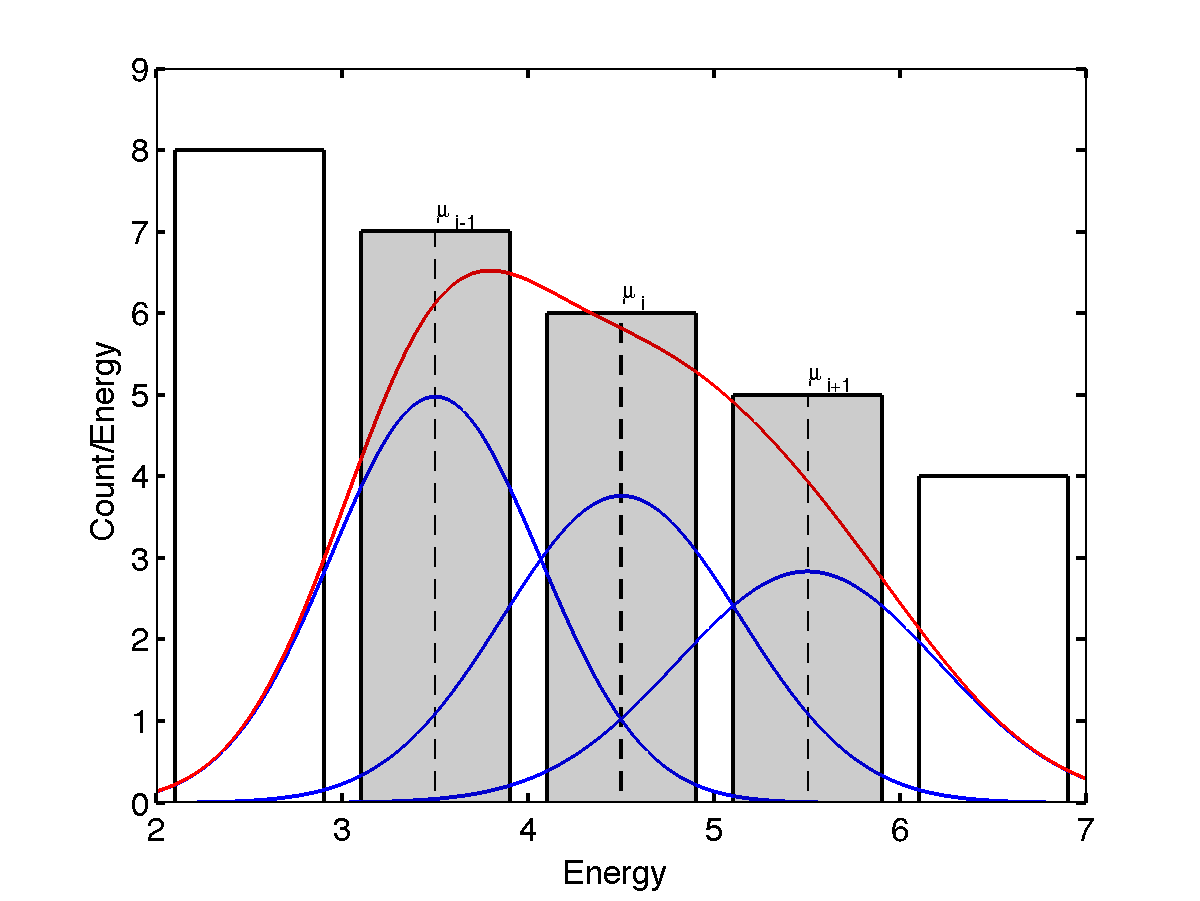
\includegraphics[width=130mm]{Chapter_Flucs/Figures/example_integral}
\caption{Smearing of a linear spectrum using equation \ref{eq:1} for an arbitrary energy scale E. The counts in each shaded bin are redistributed into normalized Gaussians (blue) with the resolution $\rm \sigma_E$ growing like $\rm \sqrt{E}$. The spectrum smeared with detector resolution is the sum of Gaussians shown in red. }
\label{fig:exp_int}
\end{figure}


\subsection{Calculating the Observed Energy}

After modeling the finite resolution with Gaussians the mean observed at each bin can be calculated from the overlap of all bins weighted by the corresponding means. We can write the observed mean in the $\rm i^{th}$ bin, $\nu_i$, in terms of the bin centers $\mu$ and overlapping areas of all bins using the normalizations $\rm c_i$ from equation \ref{eq:1}:
%\begin{center}
\begin{equation}
\nu_i = \frac{\mathlarger{\sum}\limits_{j=1}^{n}\ \mu_j\mathlarger{\int}\limits_{\mathsmaller{\mu_i-\frac{\Delta x}{2}}}^{\mathsmaller{\mu_i+\frac{\Delta x}{2}}} G_{j}(x)\,\mathrm{d}x} 
{\mathlarger{\sum}\limits_{j=1}^{n} \ \mathlarger{\int}\limits_{\mathsmaller{\mu_i-\frac{\Delta x}{2}}}^{\mathsmaller{\mu_i+\frac{\Delta x}{2}}} G_{j}(x)\,\mathrm{d}x}  
\label{eq:2}
\end{equation}
%\end{center}

Equation \ref{eq:2} can be solved in terms of error function and complimentary error function. First we will generalize a formula to solve for the overlapping area from the $\rm j^{th}$ bin into the $\rm i^{th}$ bin. 
\begin{equation}
%\rm A_i = c_i \ erf\left(\frac{\Delta x}{\sigma_i\sqrt{2}}\right) + \sum\limits_{n\neq i}^{} \frac{c_n}{2} erfc\left(\frac{|\mu_n-\mu_i| - \frac{\Delta x}{2}}{\sigma _n\sqrt{2}} \right) - 
%\sum\limits_{n\neq i}^{} \frac{c_n}{2} erfc\left(\frac{|\mu_n-\mu_i| + \frac{\Delta x}{2}}{\sigma _n\sqrt{2}} \right) 
\rm A_{i,j}=\mathlarger{\int}\limits_{\mathsmaller{\mu_i-\frac{\Delta x}{2}}}^{\mathsmaller{\mu_i+\frac{\Delta x}{2}}}\it G_{j}(x)\,\mathrm{d}x =
\begin{cases}\rm c_i \ erf\left(\frac{\Delta x}{\sigma_i\sqrt{2}}\right), & j=i  \\
\rm \frac{c_j}{2} erfc\left(\frac{|\mu_j-\mu_i| - \frac{\Delta x}{2}}{\sigma _j\sqrt{2}} \right) - 
\rm \frac{c_j}{2} erfc\left(\frac{|\mu_j-\mu_i| + \frac{\Delta x}{2}}{\sigma _j\sqrt{2}} \right) , & j \neq i \end{cases}
\label{eq:3}
\end{equation}

\noindent The error function and complementary error function are defined in equation \ref{eq:4} and the coefficient $\rm c_i$ is defined in equation \ref{eq:1}.
\begin{multline}
\\ \rm erf(x)=\frac{2}{\sqrt{\pi}} \times \int\limits_{0}^{x} exp(-t^2)\\
\rm erfc(x)=\frac{2}{\sqrt{\pi}} \times \int\limits_{x}^{\infty} exp(-t^2) = 1 - erf(x)\\
\label{eq:4}
\end{multline}


As $\rm \mu$ approaches zero the Gaussian distribution of equation \ref{eq:1} begins to spill over into negative values, which in some cases may be nonphysical. For instance, the Gaussian assumption leads to negative photons. We can chose to ignore this area or make the distribution more Poisson-like by bouncing the Gaussian back at $\rm \mu = 0$. The formula for accounting for the area of the reflected Gaussian is described in \ref{eq:6}. Ultimately this assumption has little impact on the S1 and S2 analysis because the threshold cut off well before the zero interface is reached, but it does make the distributions more Poisson like near the zeroth bins. Equation \ref{eq:6} is the same as \ref{eq:3} with the bin center $\rm \mu_i$ mapped to $\rm -\mu_i$.

\begin{equation}
%\rm A_i = c_i \ erf\left(\frac{\Delta x}{\sigma_i\sqrt{2}}\right) + \sum\limits_{n\neq i}^{} \frac{c_n}{2} erfc\left(\frac{|\mu_n-\mu_i| - \frac{\Delta x}{2}}{\sigma _n\sqrt{2}} \right) - 
%\sum\limits_{n\neq i}^{} \frac{c_n}{2} erfc\left(\frac{|\mu_n-\mu_i| + \frac{\Delta x}{2}}{\sigma _n\sqrt{2}} \right) 
\rm B_{i,j}=
\rm \frac{c_j}{2} erfc\left(\frac{|\mu_j+\mu_i| - \frac{\Delta x}{2}}{\sigma _j\sqrt{2}} \right) - 
\rm \frac{c_j}{2} erfc\left(\frac{|\mu_j+\mu_i| + \frac{\Delta x}{2}}{\sigma _j\sqrt{2}} \right)
\label{eq:6}
\end{equation}


Finally, we solve for the observed mean in the $\rm i^{th}$ bin by summing all the Gaussian overlaps $\rm A_{i,j}$ + $\rm B_{i,j}$ (equations \ref{eq:3},\ref{eq:6}), weighting the overlapping area from each bin by the corresponding bin center $\rm \mu_j$. The result is shown in equation \ref{eq:5} and is equivalent to equation \ref{eq:2} when the area from the reflected Gaussian is not considered, $\rm B_{i,j}$=0.
\begin{equation}
\rm \nu_i =  \frac{\sum\limits_{j=1}^{n}\mu_j\cdot (A_{i,j}+B_{i,j})}{\sum\limits_{j=1}^{n} (A_{i,j}+B_{i,j})}
\label{eq:5}
\end{equation}

\subsection{Smearing a Toy Spectrum}

To demonstrate the application of equation \ref{eq:5} we use it to smear a toy linearly decaying spectrum. By modifying the dependence of $\rm \sigma_i$ on $\rm \mu_i$ we can better understand the effects of the spectral shape and the functional form of the resolution.

Figure \ref{fig:Toy_Linear} shows the effect of the finite resolution on a linearly decaying spectral shape. Using a constant resolution $\rm \sigma$ the observed mean, when accounting for finite resolution, shifts down due to the spectral shape. In the case with $\rm \sigma_i \sim \sqrt{\mu_i} $ the observed mean at first shifts higher as the increasing width at higher value bin centers, even with lower counts, out weighs the lower bin centers with higher counts and narrower widths. In both cases as the bin centers approach zero the observed mean shifts higher due to an imposed threshold at zero, where Poisson statistics take over and the Gaussian characterization leads to a loss of events below zero. Thus, for the sake of the toy model in figure \ref{fig:Toy_Linear} we only characterize the relation between the real mean and the observed mean from the second bin center. It is also worth mentioning that for the case of having a varying resolution in figure \ref{fig:Toy_Linear} the shift in spectral shape seems minor, yet there is a a significant 20\% deviation in the observed mean of the last bin.

 \begin{figure}[h!]\centering
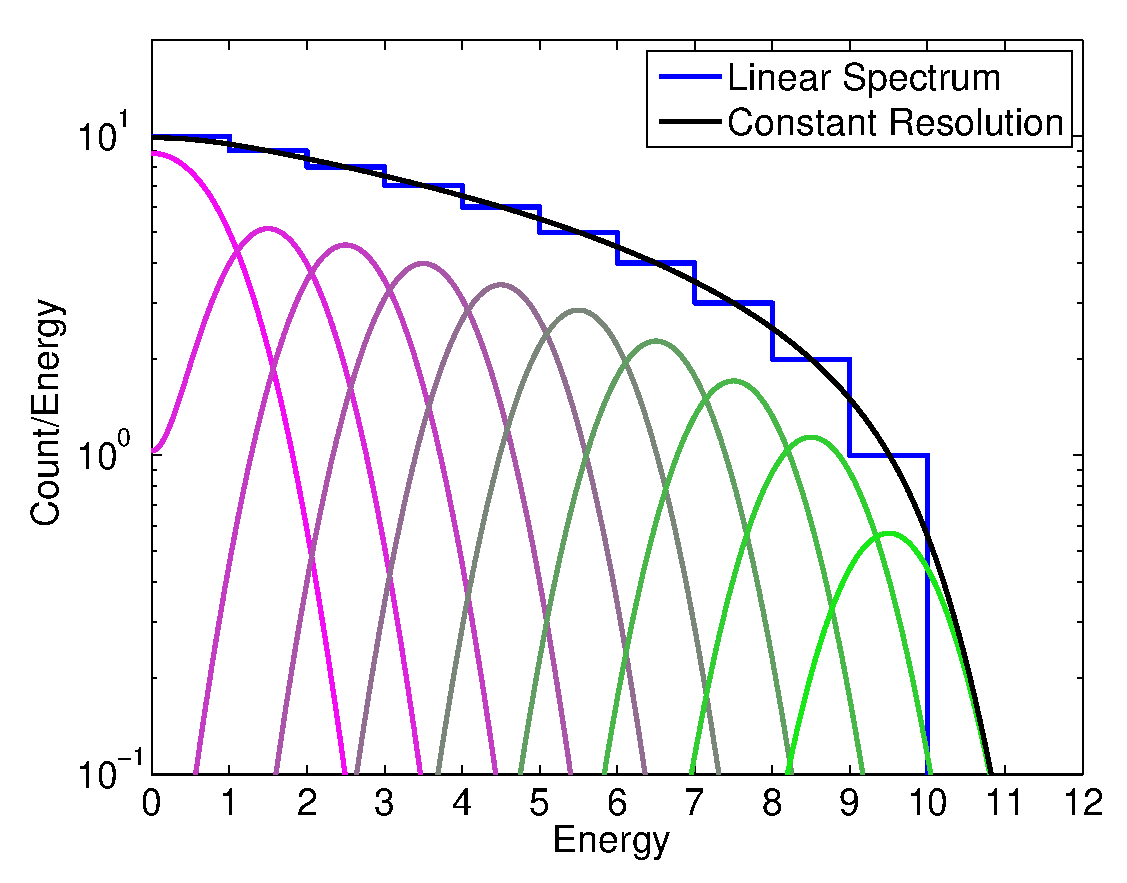
\includegraphics[width=70mm]{Chapter_Flucs/Figures/Toy_Model_lin_const}
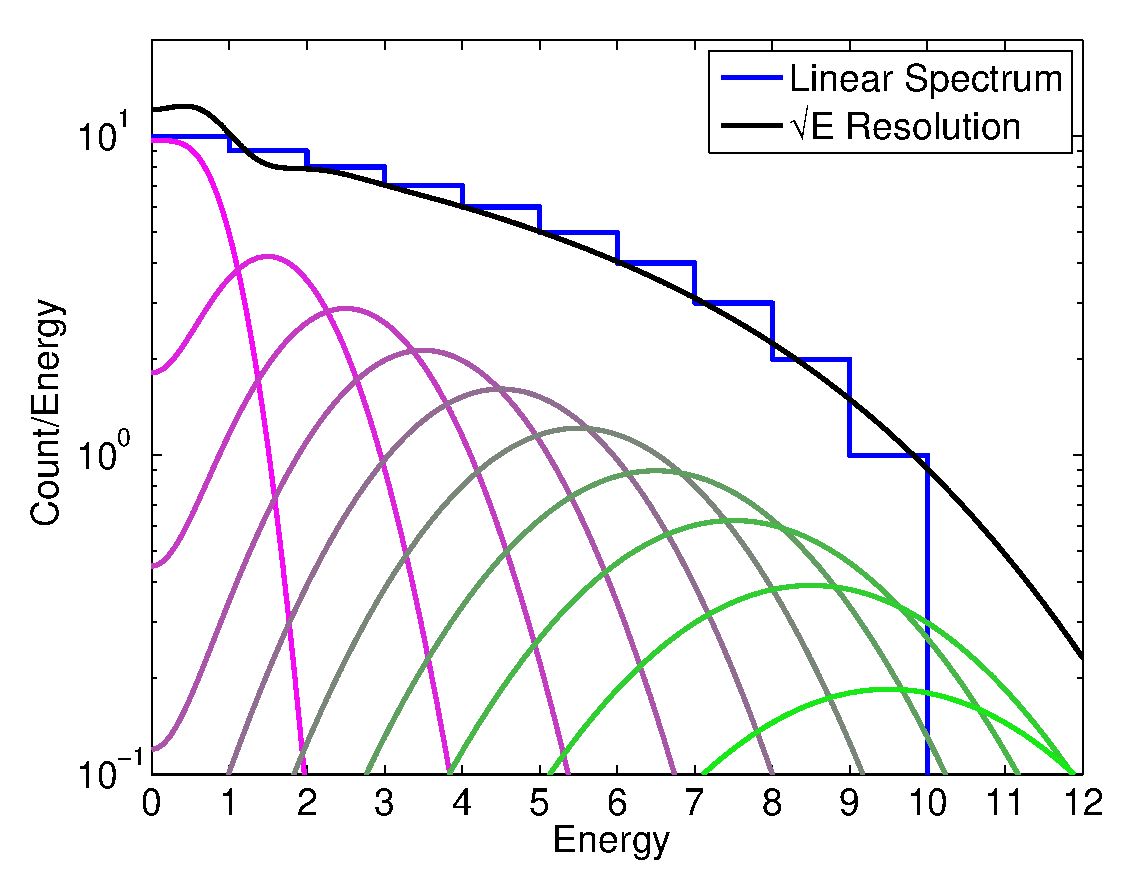
\includegraphics[width=70mm]{Chapter_Flucs/Figures/Toy_Model_lin_dep}
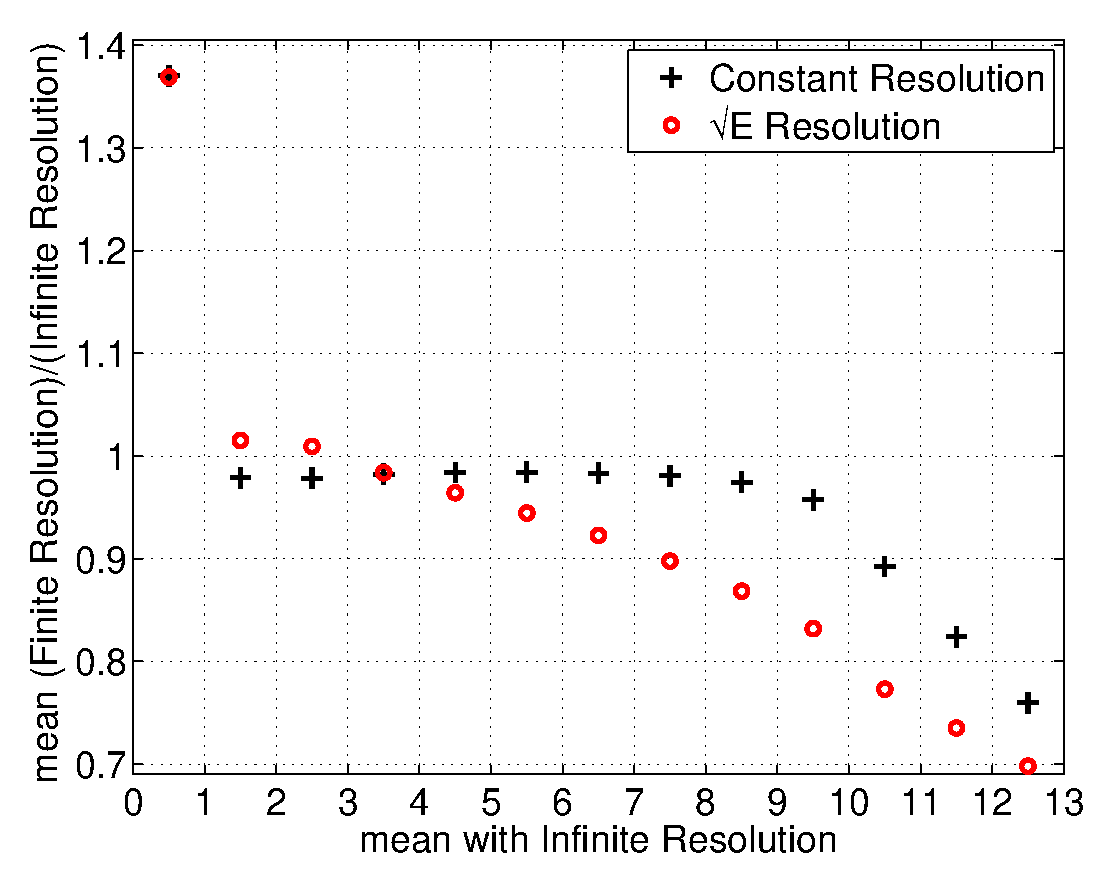
\includegraphics[width=70mm]{Chapter_Flucs/Figures/Toy_Model_mean_shift}
\caption{Top Left: A linearly decaying spectrum, in blue. The black curve represents the sum of the Gaussians assuming a constant resolution. Top Right: A linearly decaying spectrum, in blue. The black curve represents the sum of the Gaussians with a $\rm \sigma= \sqrt{E}$ dependent resolution. Bottom: The observed mean, with finite resolution, compared to the real mean with infinite resolution. The black points are for the case with linear resolution and the red points represent the case with $\rm \sigma = \sqrt{E}$ dependent resolution.}
\label{fig:Toy_Linear}
\end{figure}

\newpage



\section{Light Yield, Charge Yield and Comparison to NEST Modeling}

The first attempt to remove the effect of the tritium spectral shape and finite detector resolution is to use the NEST model from \cite{NEST_2013}. 
NEST stands for Nobel Element Simulation Technique. NEST fits data from previous xenon and argon detectors to recombination models, producing predictions for light yield $\rm n_\gamma/keV$ and charge yield ($\rm n_e/keV$) at a verity of electric fields, energy deposits, and particle types. We take the light yield (LY) and charge yields (QY) from NEST and convolve it with the known tritium energy spectrum to produce the S1 and S2 spectra. The S1 and S2 spectra are then smeared with detector resolution and recombination fluctuations, determined in chapter \ref{Ch:Flucs}. It is found  that the S1 and S2 spectra from the data deviate from the NEST model making it difficult to reverse-engineer the effect of smearing. However, taking the NEST model to be correct within 20\%, the spectral shape correction is calculated and found to be small. We proceed to extract LY, QY and recombination fluctuation ($\rm \sigma_R$) from the tritium data without any correction producing a model that is more accurate than NEST. It should be noted that the NEST model which has not been confirmed at our electric field and energy. %The extracted LY, QY and  $\rm \sigma_R$ can then be convolved with the true tritium energy spectrum and detector resolution in order to calculate a more accurate spectral shape correction.

%The first step is to solve for the value of $\rm \sigma_R$ (recombination fluctuation) that needs to be input into the smearing model, the statistical part from detector resolution remains fixed. Figure \ref{fig:R_T} show the optimal value of $\rm \sigma_R$ being extracted from the tritium data, starting with an initial guess based on the recombination fluctuation measured from the $\rm^{83m}Kr$ data.


\subsection{Tritium S1 and S2 vs. NEST}
\label{sec:Spec_Corr}

The spectral shape correction for the mean of the observed S1 and S2 signal from tritium beta decay can be found using equation \ref{eq:5}. We start with NEST to get the expected S1 and S2 tritium spectrum. The variance of S1 and S2 arise from recombination fluctuations and detector resolution (statistical and instrumental fluctuations), given in equation \ref{eq:SigStat} and \ref{eq:SigInst}. We use equations \ref{eq:S1_res} and \ref{eq:S2_res} to smear the photon and electron yields, essentially putting in detector resolution by hand. Then, by applying equations \ref{eq:1}-\ref{eq:5} the S1 and S2 bin centers after smearing can be mapped back to the true bin centers before smearing.

\begin{equation}
\begin{split}
 \rm \sigma_{S1_R}^2=g_1^2(\sigma_R^2) \\
 \rm \sigma_{S1_{Det}}^2=g_1^2(\sigma_{n_{\gamma_{stat}}}^2+\sigma_{n_{\gamma_{inst}}}^2) \\
 \rm \sigma_{S1}^2=\sigma_{S1_R}^2 + \sigma_{S1_{Det}}^2
\label{eq:S1_res}
\end{split}
\end{equation}

\begin{equation}
\begin{split}
 \rm \sigma_{S2_R}^2=g_2^2(\sigma_R^2) \\
 \rm \sigma_{S2_{Det}}^2=g_2^2(\sigma_{n_{e_{stat}}}^2+\sigma_{n_{e_{inst}}}^2) \\
 \rm \sigma_{S2}^2=\sigma_{S2_R}^2 + \sigma_{S2_{Det}}^2
\label{eq:S2_res}
\end{split}
\end{equation}

\noindent where g1 and g2 are the gains to convert S1 and S2 to number of photons and electrons, respectively. The values $\rm \sigma_{S1_R}^2$ and $\rm \sigma_{S2_R}^2$ are the variances in S1 and S2 given only recombination fluctuations, this is what a detector with infinite resolution would observe. Detector resolution is comprised of the statistical and instrumental fluctuations in light and charge collection written as $\rm  \sigma_{S1_{Det}}^2$ and $\rm  \sigma_{S2_{Det}}^2$, this would be the resolution given no recombination fluctuations. The total variance in S1 and S2 observed by a detector with finite resolution is the sum of recombination fluctuations and detector resolution $\rm \sigma^2=\sigma_{R}^2 + \sigma_{Det}^2$ (where the subscripts S1 and S2 have been removed).
The use of Gaussian sigma down to low S1 is an acceptable approximation since the underlying distribution actually consists of the number of photons, $\rm n_\gamma = \frac{S1}{g1}$. With g1=0.097 there are still 30 photons near the S1 threshold of 3 PE. The S2 threshold for golden events is around 400 PE, $\rm n_e = \frac{S2}{g2}$. With g2=5.75 there are still 70 electrons near the lower end of the tritium spectrum.

%We will use the Gaussian approximation as it makes the application of equations \ref{eq:1}-\ref{eq:5} simpler.
%The variance in S1 due to recombination fluctuations, statistical fluctuations and instrumental fluctuations at a given energy. The functional form of all three have been previously measured and can be extrapolated for use with the tritium spectrum. The first step is to use the expected light yields from NEST along with the measured smearing from recombination and detector resolution to extract a correction factor for the observed S1 signal. Having a priori knowledge of light yields will allow for the spectral shape to be corrected or can at least be used to approximate an error when we go to extract the light yield and recombination fluctuations from the tritium beta spectrum.




%The correction is calculated starring with the NEST photon and electrons yields \cite{NEST_2013}, applying the gain g1 or g2, and convolving it with a tritium beta spectrum along with our approximation of recombination fluctuations measured in equation \ref{eq:Inst_Fit}. 

Figure \ref{fig:S1S2_mapping} (a,c) shows the application of smearing from equation \ref{eq:S1_res} and \ref{eq:S2_res} to the expected S1 and S2 tritium spectrum, respectively, overlaid with the data. The mapping of the observed S1 and S2 mean values to the real S1 and S2 mean values is shown in \ref{fig:S1S2_mapping} (b,d). The mapping from observed mean to real mean is the result of starting with infinite resolution containing recombination fluctuations only ($\rm \sigma_R$) and applying the model as outlined in \ref{sec:Smear} with detector resolution ($\rm \sigma_{Det}$ of equations \ref{eq:S1_res} and \ref{eq:S2_res}). 
%Applying the correction factor to the data reveals the mean S1s that the LUX detector would observe given infinite detector resolution.

% S1 S2 result NEST iter 0
\renewcommand{\baselinestretch}{1}
\small\normalsize
\begin{figure}[h!]\centering
 
\subcaptionbox{S1 \label{fig:5a}}{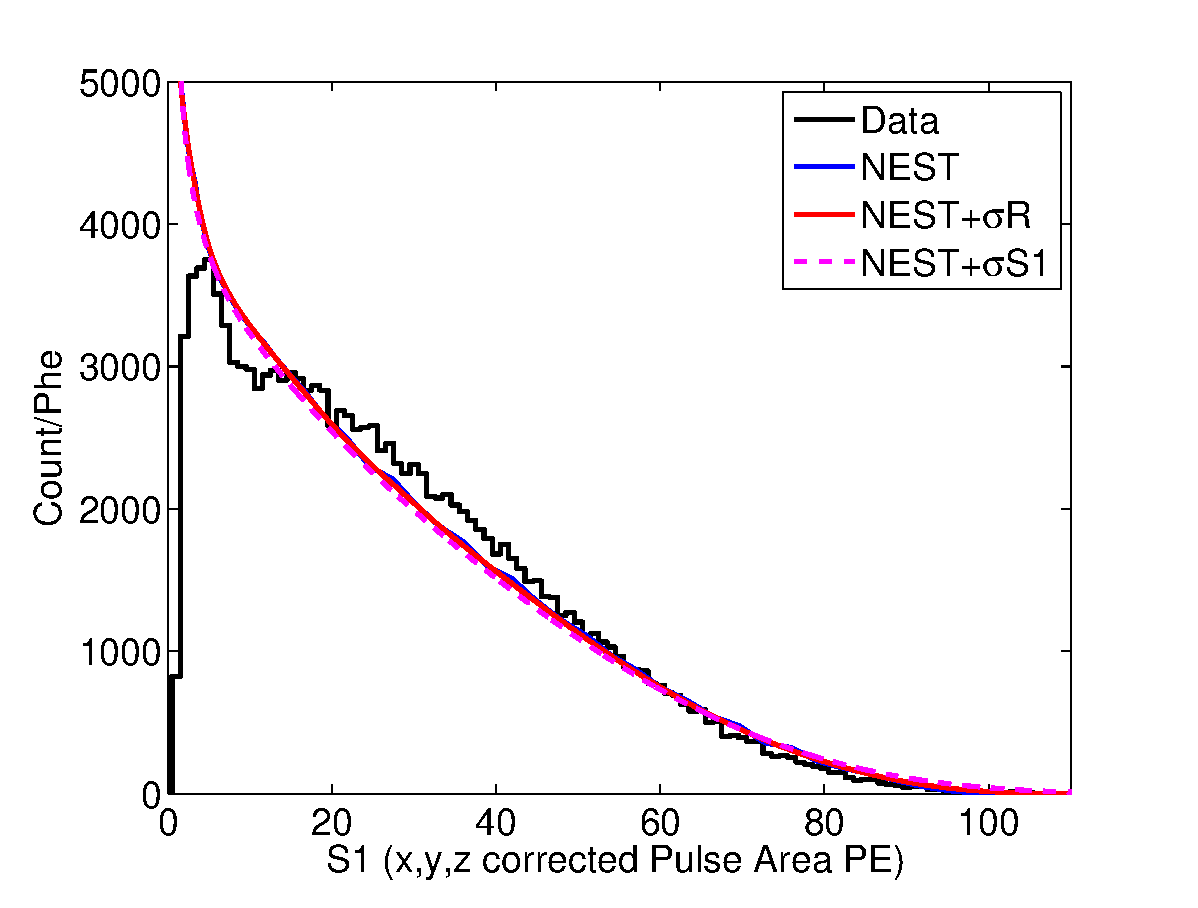
\includegraphics[width=73mm]{Chapter_Flucs/Figures/S1S2_Spectra/S1_spec_compare_.eps}}
\hfill
\subcaptionbox{S1 \label{fig:5b}}{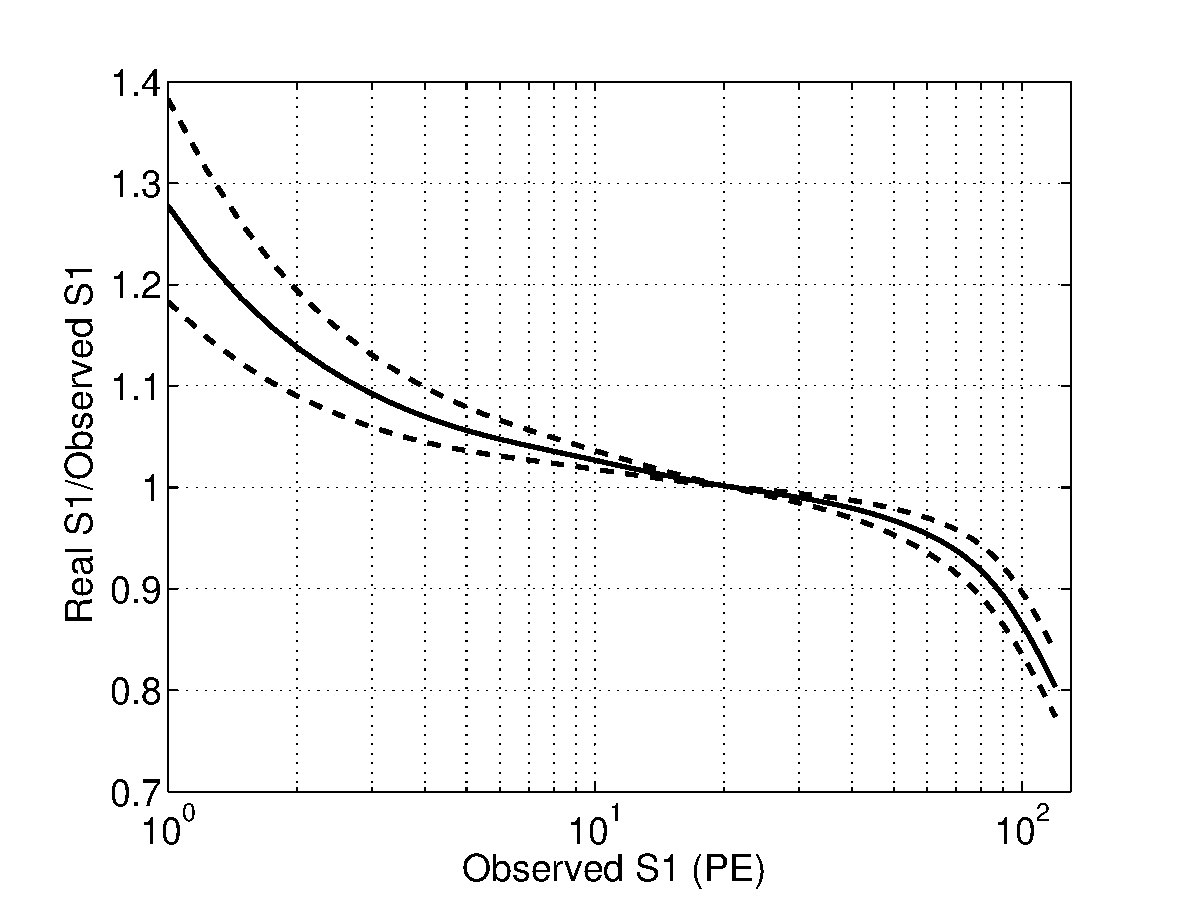
\includegraphics[width=73mm]{Chapter_Flucs/Figures/S1S2_Spectra/S1_corr_.eps}}

\bigskip

\subcaptionbox{S2 \label{fig:5c}}{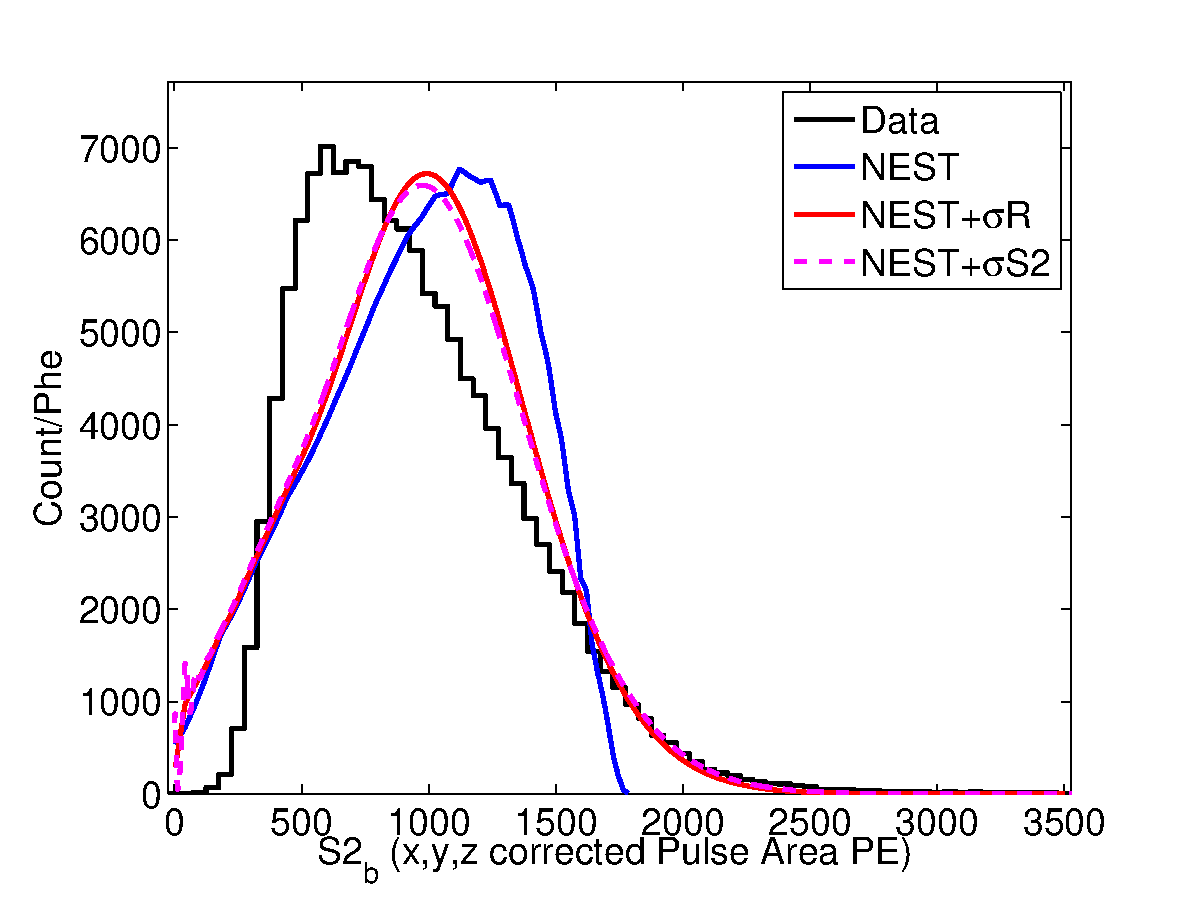
\includegraphics[width=73mm]{Chapter_Flucs/Figures/S1S2_Spectra/S2_spec_.eps}}
\hfill
\subcaptionbox{S2 \label{fig:5c}}{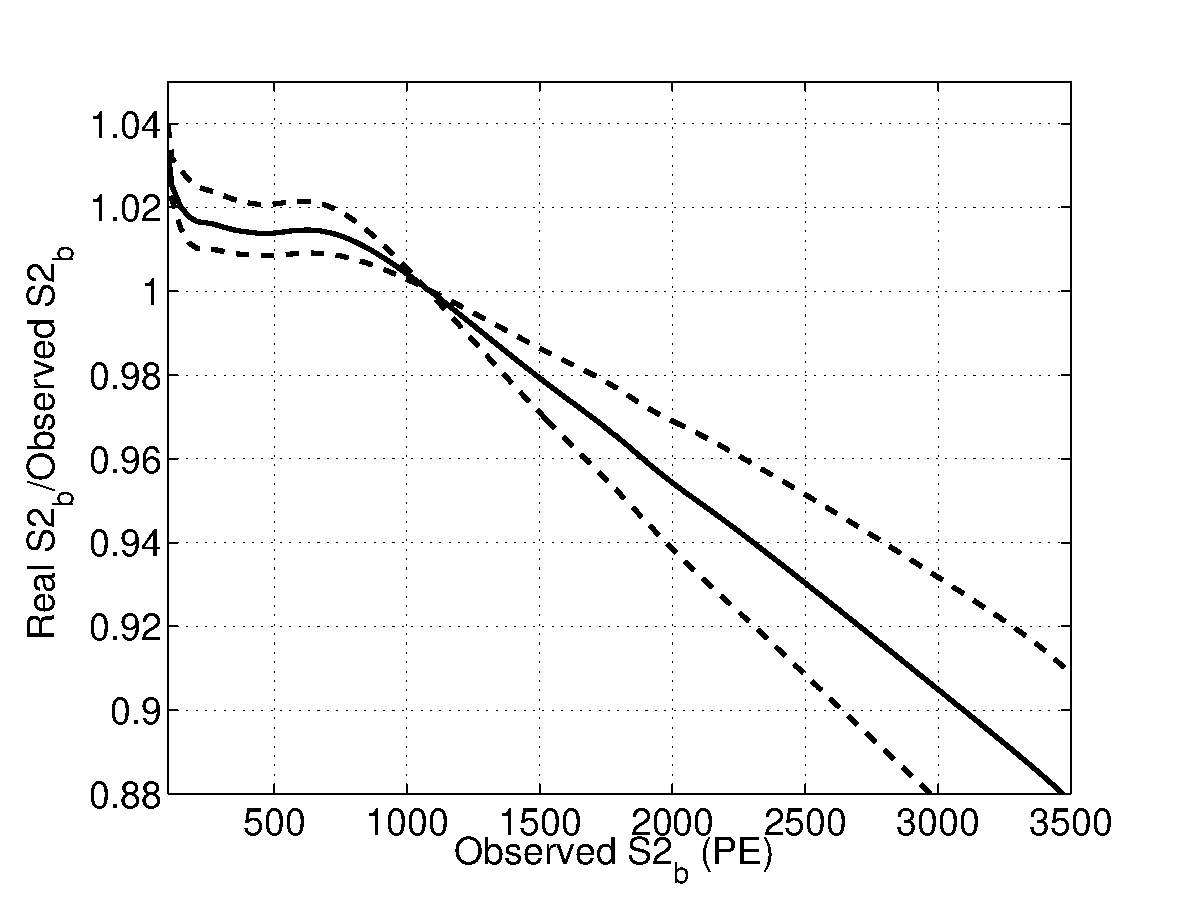
\includegraphics[width=73mm]{Chapter_Flucs/Figures/S1S2_Spectra/S2_corr_.eps}}

\caption{ a): In Black S1 tritium S1 spectrum extracted from the data. In blue, The NEST light yield curve. In red, the NEST light yield curve with recombination fluctuations. Dashed magenta is NEST light yield with smearing from equations \ref{eq:S1_res}.  b): The ratio of the real S1 mean to the S1 observed mean vs. the observed mean after smearing. Note, the S1 threshold at about 3 PE in S1. c): In Black S2 tritium spectrum extracted from the data. In blue, The NEST light yield curve. In red, the NEST light yield curve with recombination fluctuations. Dashed magenta is NEST light yield with smearing from equations \ref{eq:S2_res}.  d): The ratio of the real S2 mean to the S2 observed mean vs. the observed mean after smearing. }

\label{fig:S1S2_mapping}
\end{figure}
\renewcommand{\baselinestretch}{2}
\small\normalsize


We find that that peak location of the S2 spectra from NEST deviates from the data by up to 20\%. These discrepancies maybe arising from the error  in g1 and g2 which could systematically shift light yield and charge yield by the appropriate amount. However, modifying g1 and g2 only induces a horizontal shift left or right, and the data indicates the need to modify the derivative of LY and QY from NEST.

 
Since the means of the model do not line up with the data the calculated corrections in figure \ref{fig:S1S2_mapping} can't be applied. In order to account for detector resolution as outlined in section \ref{sec:Smear} we must have a reasonably accurate initial guess of the spectrum with infinite resolution. In this case we do not. However, even though the means from NEST light and charge yields are off we find that the effect of recombination fluctuations and detector resolution is relatively small. The correction for the S1 ranges from +30\% to -20\% and the S2 correction from +2\% to -10\%. We takes these as small enough to proceed with extracting light yield, charge yield and recombination without any correction in order to construct a more accurate model than our initial NEST prediction. Having outlined a method for mapping the observed S1 and S2 means to their real values we will now gauge the effect of finite resolution on the observed total energy.  %since we are interested in measuring quanta per bin of energy.



\begin{comment}
 \begin{figure}[h!]\centering
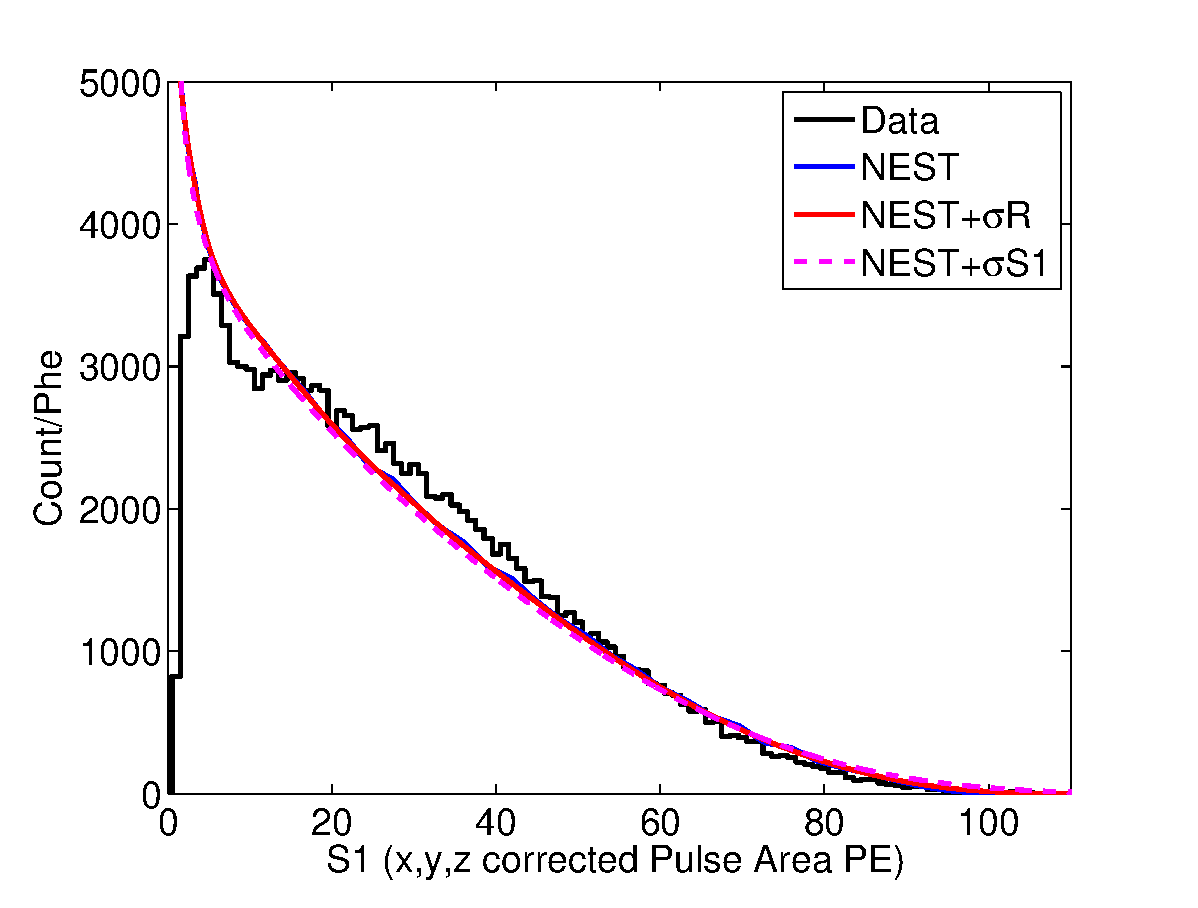
\includegraphics[width=70mm]{Chapter_Flucs/Figures/S1S2_Spectra/S1_spec_compare_.eps}
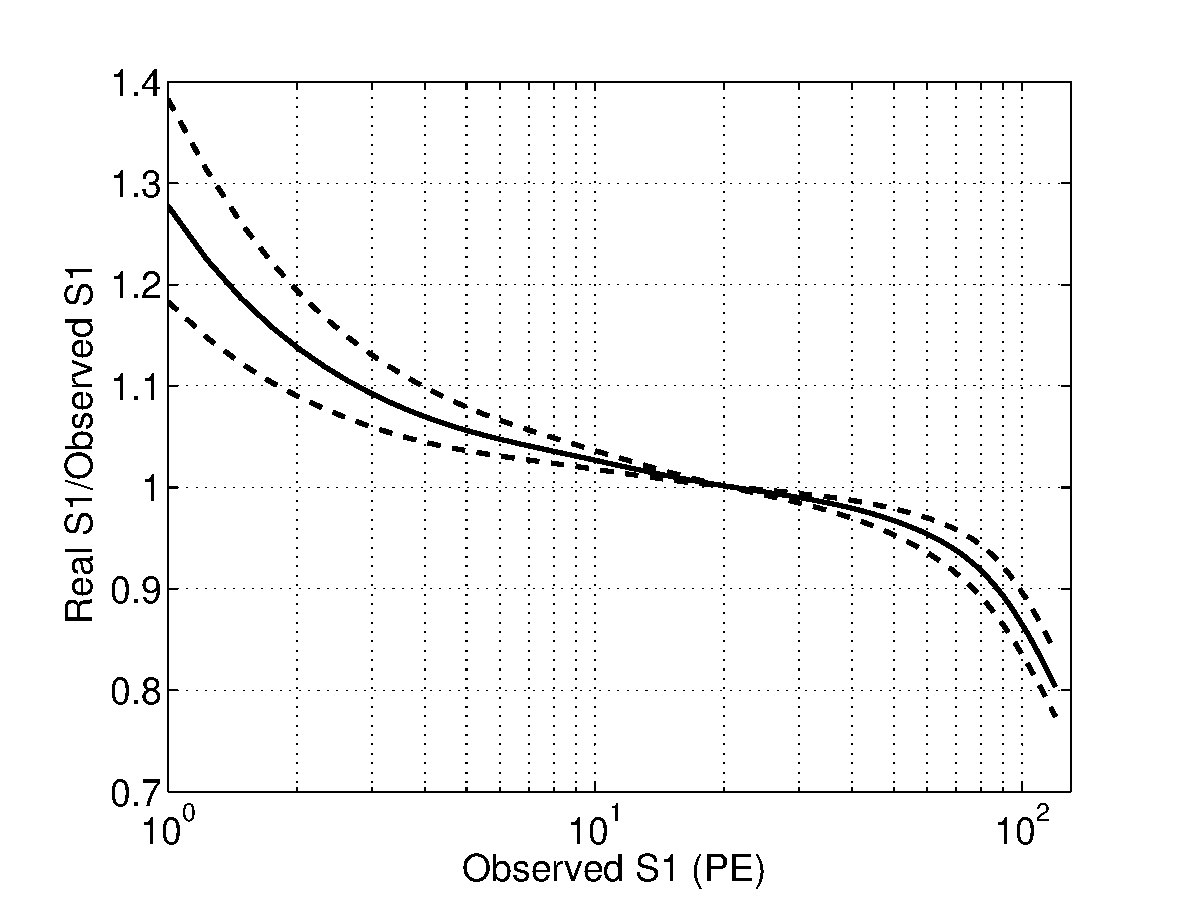
\includegraphics[width=70mm]{Chapter_Flucs/Figures/S1S2_Spectra/S1_corr_.eps}
\caption{Left: In Black S1 tritium spectrum extracted from the data. In blue, The NEST light yield curve. In red, the NEST light yield curve with recombination fluctuations. Dashed magenta is NEST light yield with smearing from equations \ref{eq:S1_res}.  Right: The ratio of the real mean to the observed mean vs. the observed mean for a tritium photon spectrum. Note the S1 threshold at about 3 PE in S1. }
\label{fig:S1_mapping}
\end{figure}

 \begin{figure}[h!]\centering
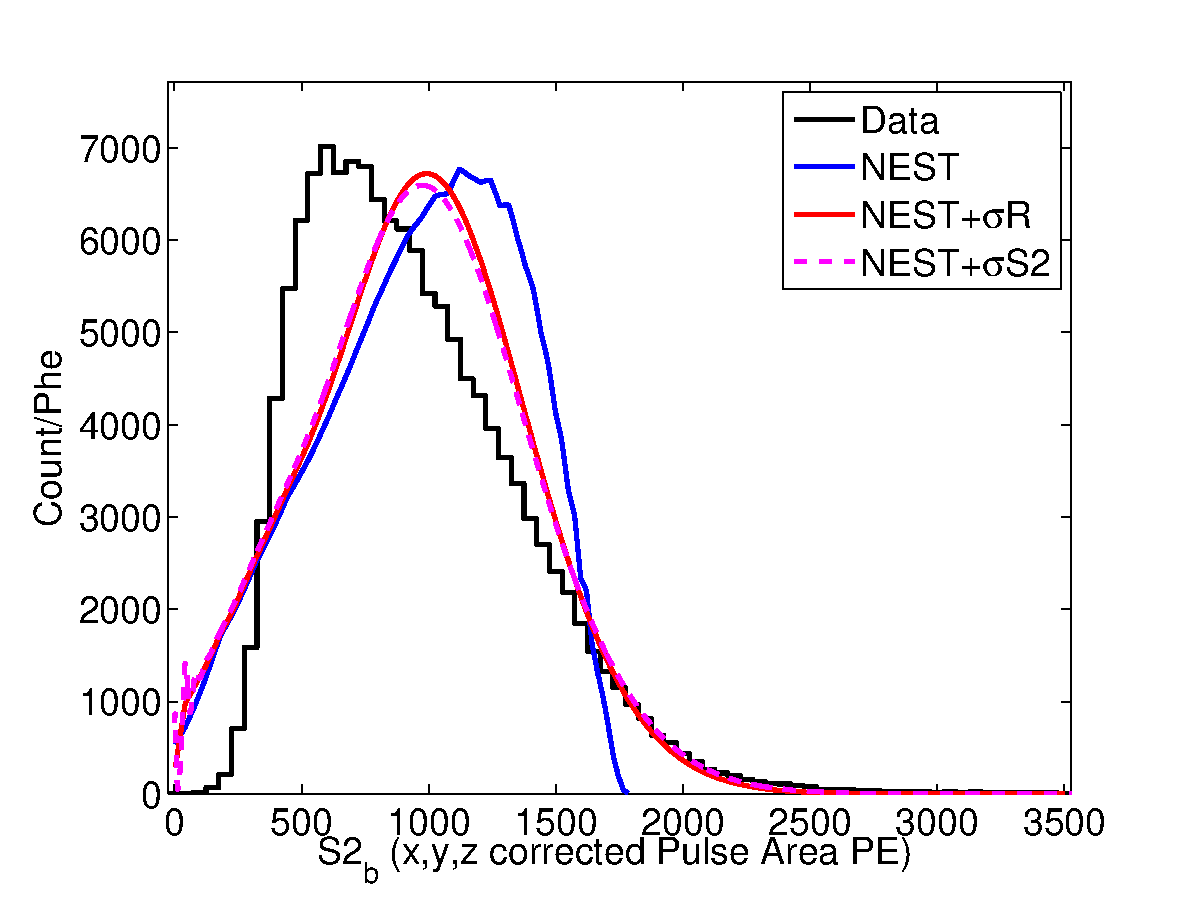
\includegraphics[width=70mm]{Chapter_Flucs/Figures/S1S2_Spectra/S2_spec_.eps}
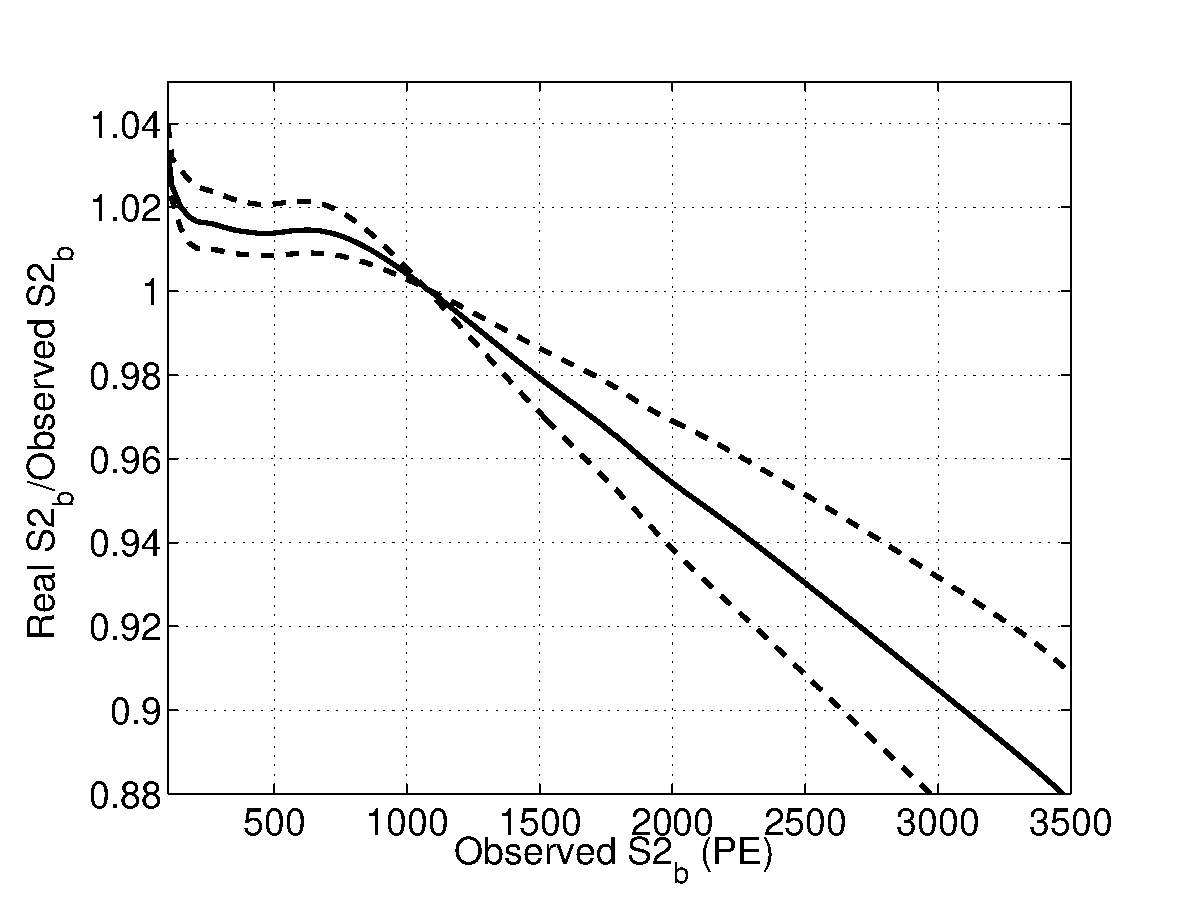
\includegraphics[width=70mm]{Chapter_Flucs/Figures/S1S2_Spectra/S2_corr_.eps}
\caption{Left: In Black S2 tritium spectrum extracted from the data. In blue, The NEST light yield curve. In red, the NEST light yield curve with recombination fluctuations. Dashed magenta is NEST light yield with smearing from equations \ref{eq:S2_res}.  Right: The ratio of the real mean to the observed mean vs. the observed mean for a tritium photon spectrum. }
\label{fig:S2_mapping}
\end{figure}
\end{comment}

%\subsection{Tritium S2 Mean and NEST}

%The correction for the mean of the measured charge yield, S2 PE, for tritium beta decay can be solved for using equation \ref{eq:5}. Starting with a simulated S2 tritium spectrum with infinite resolution and applying equations \ref{eq:1}-\ref{eq:5} one can attain the mapping of measured mean to true mean.  The resolution of S2 was determined from statistical and  instrumental fluctuations and is given in equation \ref{eq:SigStat} and \ref{eq:SigInst}. The use of Gaussian error down to low S2 is an acceptable approximation since the S2 spectrum ends at 300 PE, $\rm n_e = \frac{S2}{g2}$. With g2=5.75 there are still 50 electrons near end of the tritium spectrum, thus the Gaussian model is still a close approximation of the underlying Poisson distribution. We will use the Gaussian approximation as it makes the application of equations \ref{eq:1}-\ref{eq:5} much simpler.
%As in the case of the light yield, the variance in S2 is the result of recombination fluctuations, statistical fluctuations and instrumental fluctuations at a given energy. The functional form of all three have been previously measured and can be extrapolated for use with the tritium spectrum. We first use the expected charge yields from NEST along with the measured smearing from recombination and detector resolution to extract a correction factor for the observed S2 signal. Having a priori knowledge of light yields will allow for the spectral shape to be corrected or can at least be used to approximate an error when we go to extract the charge yield and recombination fluctuations  from the tritium beta spectrum.






\subsection{Tritium Energy Spectrum}

Unlike the S1 and S2 spectra which are dependent on light and charge yield, the tritium energy spectrum is well known \cite{Tritium_Eq}. The tritium spectrum is perhaps the most studied beta spectra, so there is no need to rely on modeling.  Also, recombination fluctuations cancel out in combined energy space leaving only detector resolution to be applied for smearing, given equation \ref{eq:E_res}. The accuracy of the smearing model described in equations \ref{eq:1}-\ref{eq:5} can be tested by comparing it against the energy observed after a full simulation, which accounts for detector geometry and having been processed by the full offline framework. Using equation \ref{eq:Fano}, \ref{eq:Gain} and \ref{eq:E_res1} we solve for the the variance of E ($\rm \sigma_{E}^2$),
%The energy depends on both S1 and S2 thus, mapping observed energy to true energy my be non-trivial.
\begin{gather}
\label{eq:E_res1} \rm E= W(n_\gamma + n_{e^-}) \\
 \rm \sigma_{E}^2= W^2(\sigma_{n_\gamma}^2 + \sigma_{n_{e^-}}^2) \\ 
 \rm \sigma_{E}^2= W^2(a_\gamma^2 n_\gamma + a_e^2 n_{e^-})
\label{eq:E_res}
\end{gather}

\noindent W is the work function $0.0137\pm0.002 \rm \frac{keV}{N_{quanta}}$, $\rm n_\gamma$ and $\rm n_e$ and number of photons and electrons respectively. The constants $\rm a_\gamma$ and $\rm a_e$ represent the coefficients of the $\rm \sqrt{n}$ term for the statistical uncertainty given in equation \ref{eq:SigStat}. There is also an instrumental component which is proportional to $\rm n_\gamma$ and $\rm n_e$. However, the instrumental term is sub-dominant at the low tritium energies with coefficients given in equation \ref{eq:SigInst}.

Starting with the tritium energy spectrum with infinite resolution we apply the empirically determined resolution in equation \ref{eq:E_res}. Figure \ref{fig:E_spec} shows the comparisons of the true tritium spectrum, the spectrum with smearing from equation \ref{eq:E_res}, the expectation from LUXSIM and the data. The smearing from the model described in equations \ref{eq:1}-\ref{eq:5} is found to be almost identical to the output of LUXSIM.

\newpage

 \begin{figure}[h!]\centering
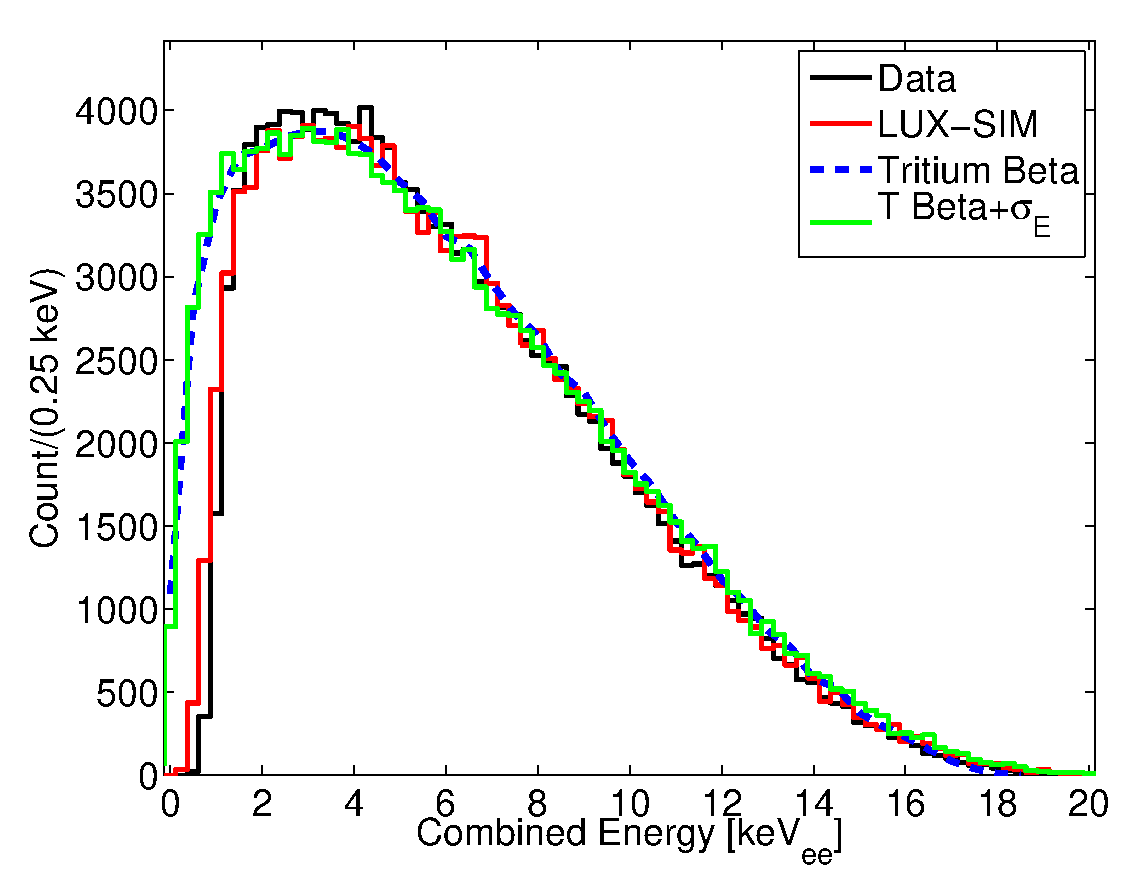
\includegraphics[width=70mm]{Chapter_Flucs/Figures/E_Spec/E_spec_compare_SIM.eps}
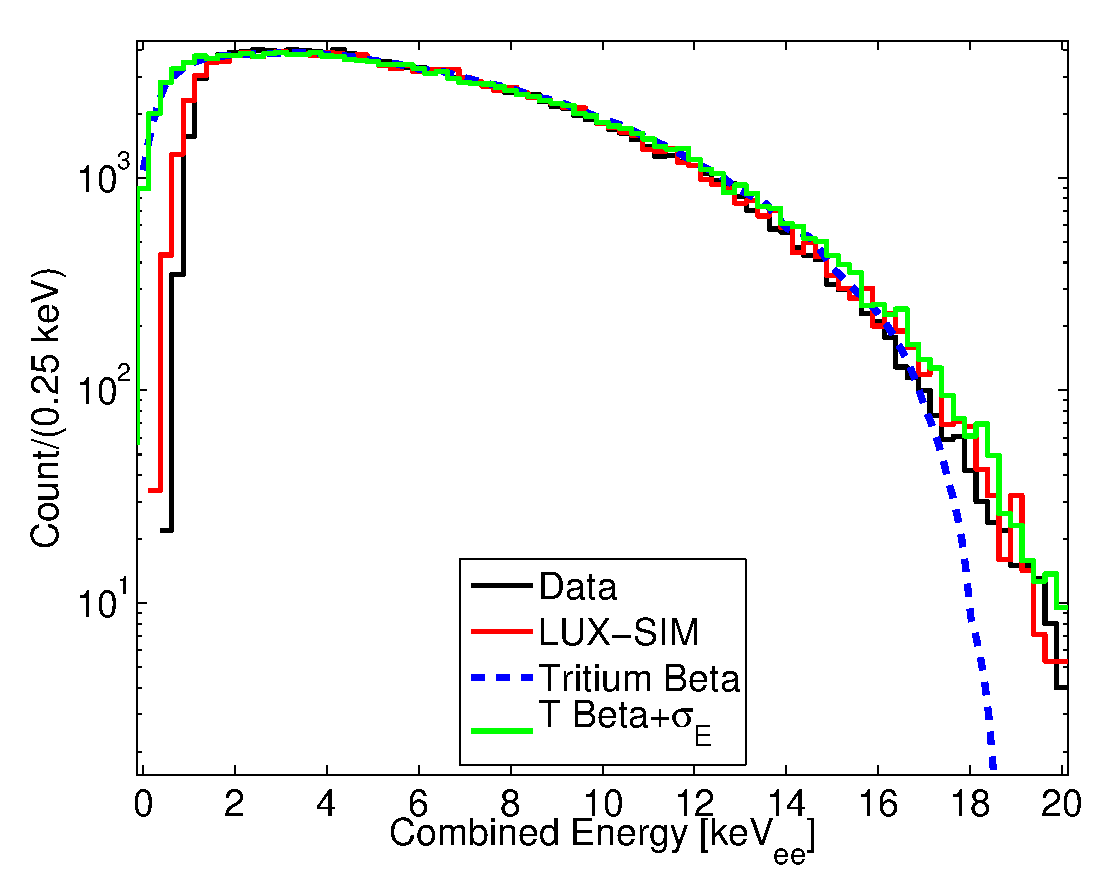
\includegraphics[width=70mm]{Chapter_Flucs/Figures/E_Spec/E_spec_compare_SIM_log_.eps}
\caption{The tritium energy spectrum reconstructed from the data (black). Along with LUX SIM (red), the true tritium beta spectrum (dashed blue) and a tritium spectrum smeared with detector resolution of equation \ref{eq:E_res} (green). }
\label{fig:E_spec}
\end{figure}

Comparing the true tritium spectrum, the data, LUXSIM and the spectrum with  \ref{eq:E_res}, we find that for the cases with finite resolution the endpoint flare out  above 16 keV. With the endpoint reaching out past 20 keV instead of terminating at 18.6 keV. This effect is precisely what the modeling in section \ref{sec:Smear} attempts to undo. Clearly events observed at 20 keV must has fluctuated up from bins below the tritium endpoint at 18.6 keV \cite{Tritium_Q}. Most importantly, besides the additional fluctuation around the endpoint the difference in spectral shape after accounting for finite resolution is hardly noticeable.


The mapping for observed energy to true energy is calculated for both LUXSIM and the simpler smearing model of equation \ref{eq:E_res}. From the LUXSIM data the initial Monte Carlo values of each event are compared to the final reconstructed energies. Each energy deposit is simulated with photon and electron propagation along with light collection in the LUX detector. Figure \ref{fig:E_mapping} shows the results for mapping observed energy to real energy using both smearing methods. 

 \begin{figure}[h!]\centering
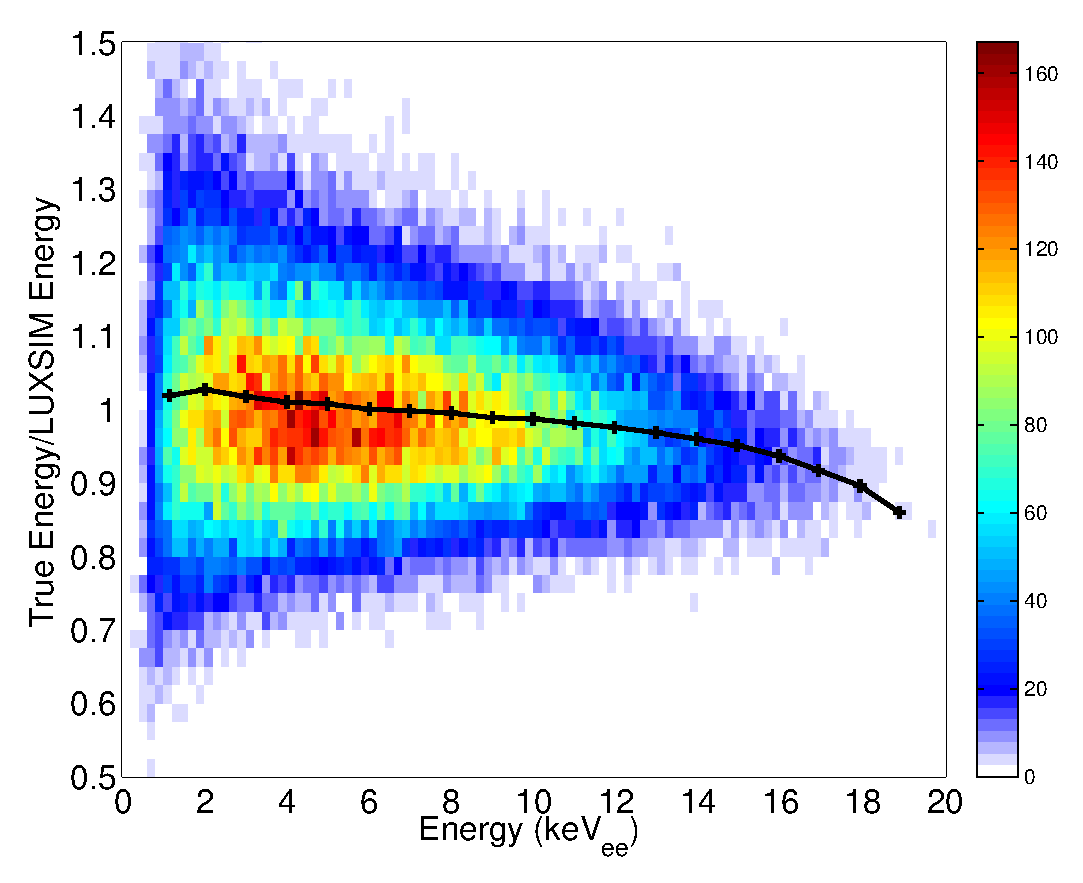
\includegraphics[width=70mm]{Chapter_Flucs/Figures/E_density_LUX_SIM_Tritium.eps}
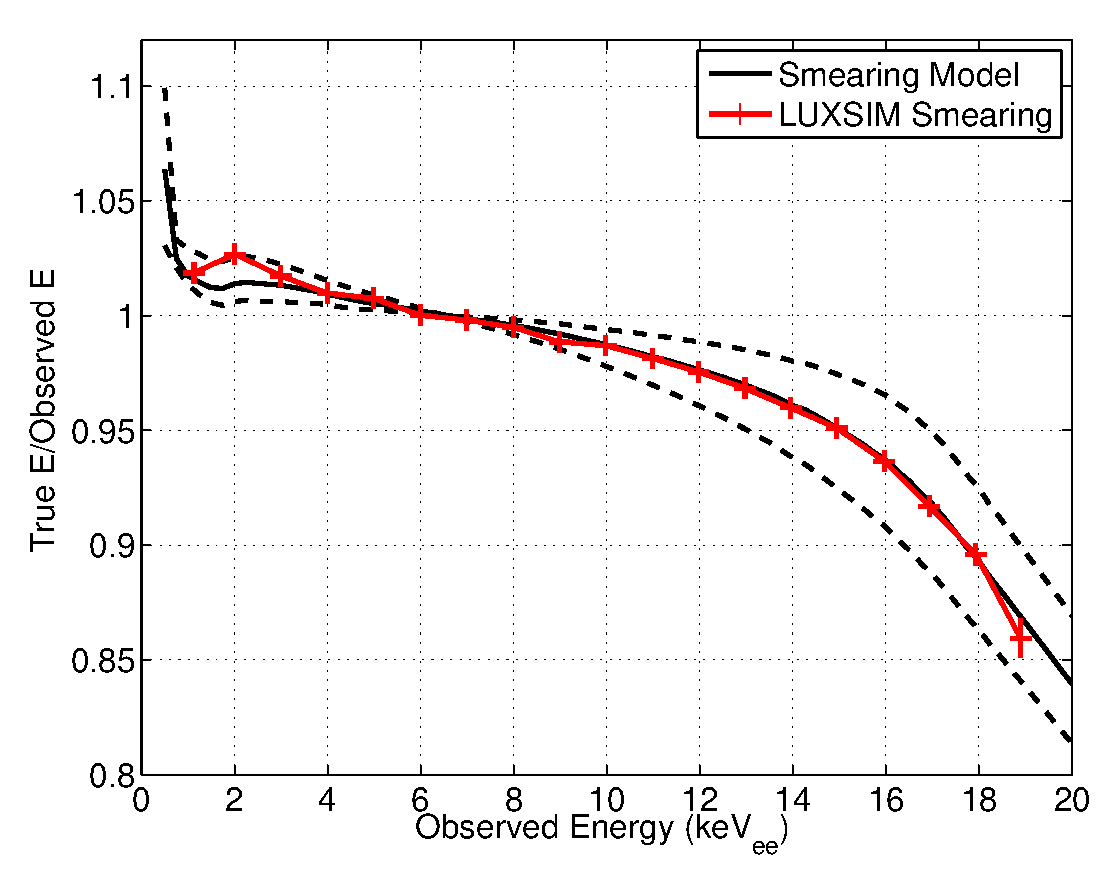
\includegraphics[width=70mm]{Chapter_Flucs/Figures/E_corr.eps}
\caption{Left, mapping from real Monte Carlo energy to observed energy plotted vs the observed energy after applying a finite resolution using LUXSIM. Right, comparing the correction determined from the Monte Carlo (Red) to the detector smearing model (black) given in equation \ref{eq:E_res}. The dashed lines represent the uncertainty in the measured values. The agreement is within errors from 1 to 18 $\rm keV_{ee}$. The Energy threshold is 50\% at 1.0 $\rm keV_{ee}$.}
\label{fig:E_mapping}
\end{figure}

The shift in the observed mean from the true mean for both LUXSIM and the model of equation \ref{eq:E_res} are in good agreement down to the threshold of 1.5 keV, the agreement with simulation is always within 1\%. Below 2 keV the model predicts the ratio of true energy to observed energy to rise as there are greater number of events at higher energy spilling over to lower energy. The simulation however does not show this behavior leading to a 5\% discrepancy in the 1 keV bin. Comparing the modeled detector resolution to the more complex LUXSIM simulations provides a proof of principle of the model.

The effect of detector resolution on skewing the true energy to observed energy is found to be minor, blowing up only at the tail end of the tritium spectrum. Over 95\% of the tritium event occur between 1 and 15 keV were the correction is less than 5\%. With this information we proceed with extracting light and charge yields without concern about incorrectly assigning the energy bin.


\subsection{Results for Light Yield, Charge Yield and Recombination}

As shown in figure \ref{fig:S1S2_mapping} the S1 and S2 spectral shape is not a good match with the light yield model from NEST, thus applying a correction to the observed means using NEST is not prudent. Fortunately, both for the S1 and S2 the spectral shape correction is less than 10\% in the region where the vast majority of the tritium events are populated. Further, the reconstructed energy is also valid to within 5\%. Knowing this we can move forward with extracting a more accurate light yield and recombination fluctuations. % accepting the small error in order to create a more accurate model than NEST to which then we can calculate the spectral shape correction.


By the same method outlined in section \ref{sec:Recomb_Data}, the number of photons, electrons and recombination fluctuation is extracted from the tritium data. This is the result of the raw data uncorrected for the spectral shape. The result is shown in figure \ref{fig:Rec_0}.

 \begin{figure}[p!]\centering
 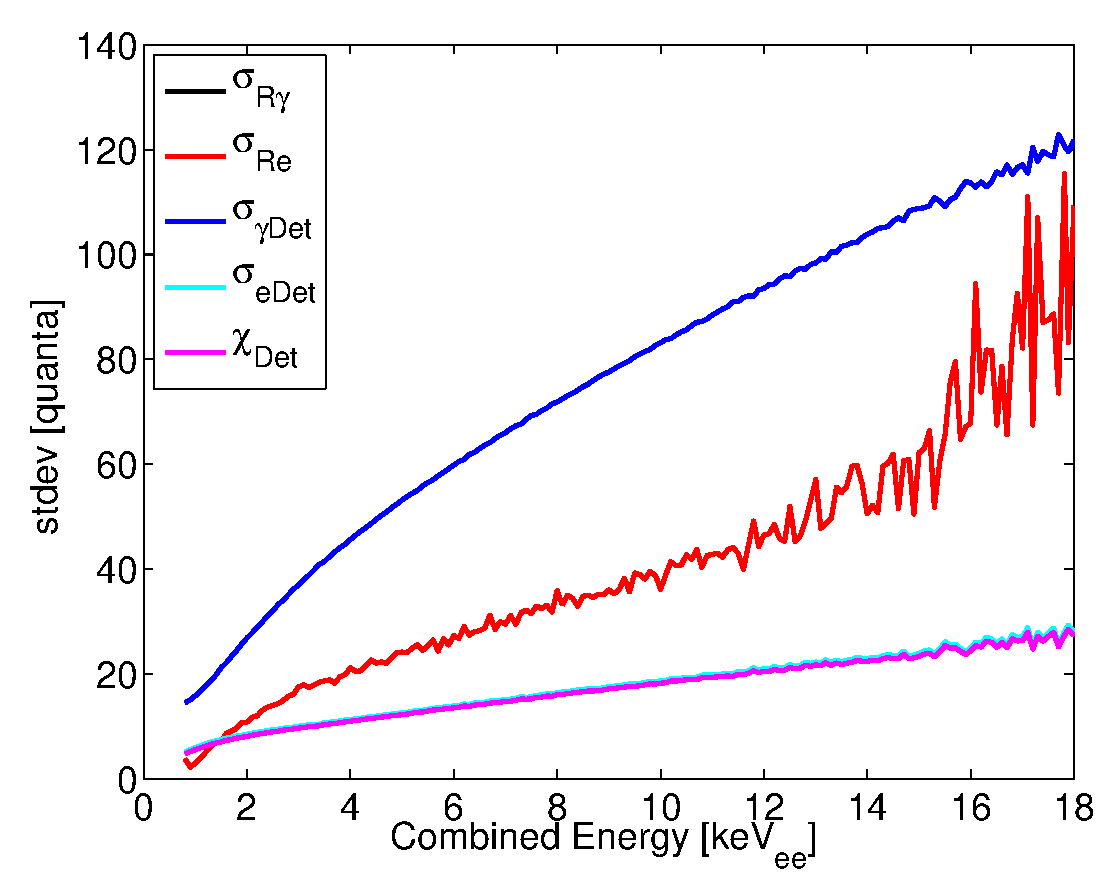
\includegraphics[width=90mm]{Chapter_Flucs/Figures/Iter0/std_fig_.eps}
 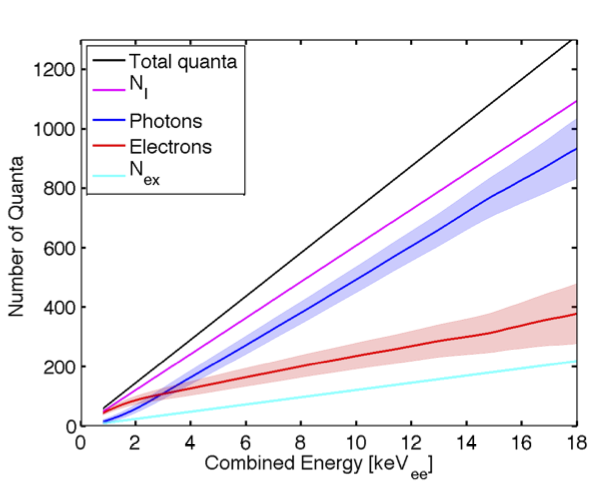
\includegraphics[width=72mm]{Chapter_Flucs/Figures/Iter0/quanta_.png}
 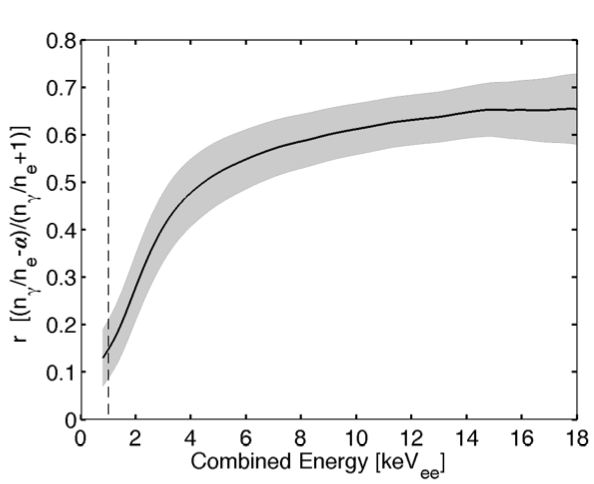
\includegraphics[width=72mm]{Chapter_Flucs/Figures/Iter0/R_.png}
\caption{Top: Extracted recombination fluctuation from the tritium data from fluctuations in photons and electrons (Black and Red respectively). Bottom right: mean number of quanta in photons, electrons, ions, excitons vs. energy keV for the tritium calibrations. Bottom left: Recombination fraction and the one sigma (shaded) vs. energy keV. The exciton-to-ion ratio is assumed to be $\rm \alpha =$ 0.20.}
\label{fig:Rec_0}
\end{figure}

Having measured number of photons, electrons in each energy bin we compare the tritium data to NEST yields, shown in figure \ref{fig:LYQY_iter0}. The disagreement between the data and the NEST yields was expected since before the S1 and S2 tritium spectrum did not line up, shown in figure \ref{fig:S1S2_mapping} . Though the means do not match the measured light yield is within 1 sigma considering the large systematic uncertainty in gains g1 and g2.  The figure also shows the one sigma prediction of the yields from NEST \cite{NEST_2013} shaded in blue where the model is interpolated and magenta where the model is extrapolated. 


%LY QY result iter 0

\renewcommand{\baselinestretch}{1}
\small\normalsize
\begin{figure}[h!]\centering
 
\subcaptionbox{$\rm n_\gamma$, 170 V/cm \label{fig:5a}}{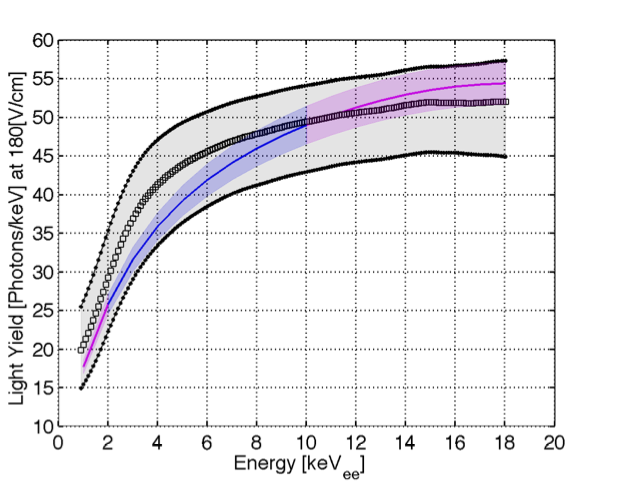
\includegraphics[width=73mm]{Chapter_Flucs/Figures/LYQY/LY_180_1sigBand_.png}}
\hfill
\subcaptionbox{$\rm n_e$, 170 V/cm \label{fig:5b}}{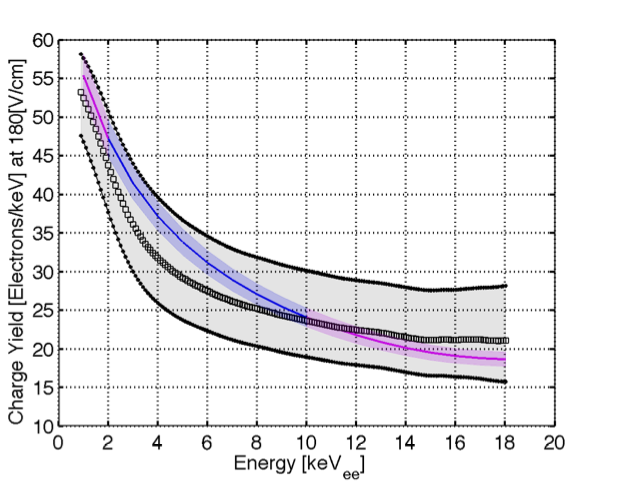
\includegraphics[width=73mm]{Chapter_Flucs/Figures/LYQY/QY_180_1sigBand_.png}}

\bigskip

\subcaptionbox{$\rm n_\gamma$ 100 V/cm \label{fig:5c}}{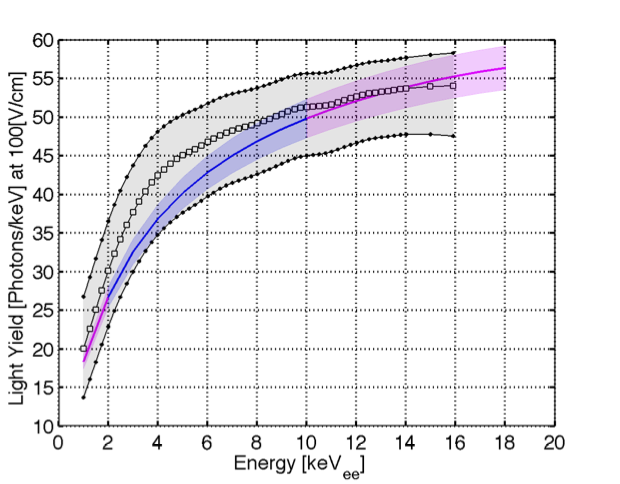
\includegraphics[width=73mm]{Chapter_Flucs/Figures/LYQY/LY_100_1sigBand_.png}}
\hfill
\subcaptionbox{$\rm n_e$, 100 V/cm \label{fig:5c}}{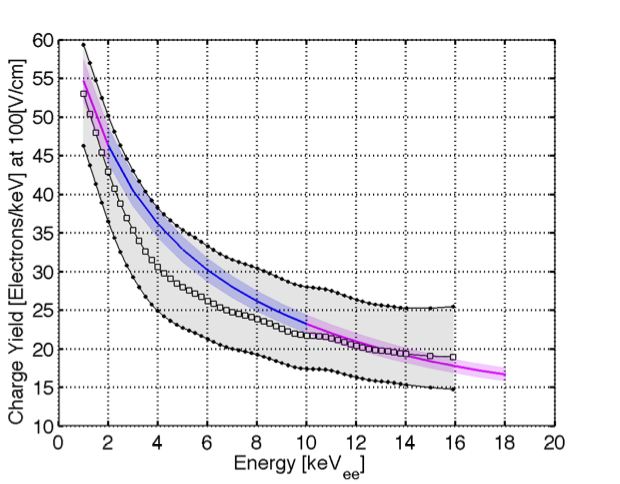
\includegraphics[width=73mm]{Chapter_Flucs/Figures/LYQY/QY_100_1sigBand_.png}}

\caption{Light yield and charge yield from tritium data without spectral shape correction at 170 V/cm in black. The shaded region represents the one sigma systematic uncertainty on g1 and g2. The NEST yield prediction and its corresponding 1 sigma is shaded in blue. NEST interpolation in show in magenta to energies where the model is not vetted. Note that the statistical errors are about the size of the data points and the dominant uncertainty illustrated by the shaded region is 100\% correlated bin-to-bin. A one sigma shift up in light yield corresponds to a one sigma shift down in charge yield and visa versa.}
\label{fig:LYQY_iter0}
\end{figure}
\renewcommand{\baselinestretch}{2}
\small\normalsize

The yields and recombination fluctuations measured from the tritium data can be used to construct an improved model over the initial NEST prediction. As mentioned previously, the effect of detector resolution can be ignored in the region where the vast majority of the tritium events occur. Having built a new model for yields we now proceed to patch up the 20-30\% shifts which occur at the edges of the S1 and S2 tritium spectra.



\section{Measuring Light Yield, Charge Yield and Recombination, Corrected for Spectral Shape}

Using the light yield and charge yield measurements extracted from the uncorrected tritium data we improve the light yield and charge yield model over the initial NEST-based model. In this section we will take the information gathered in the previous section to calculate the spectral shape correction for the tritium S1 and S2. With the improved model for LY and QY we can determine the efficiency for detecting S1s, S2s and the energy threshold. Finally, after applying the correction we can extract the true light yield and charge yield information from the tritium data.

\subsection{Tritium S1 and S2 Correction}

We now proceed to calculate the spectral shape correction using the method outlined in section \ref{sec:Spec_Corr} with NEST yields replaced by those measured from the uncorrected tritium data. Figure \ref{fig:S1S2_mapping_2} (a,c) shows the application of smearing from equation \ref{eq:S1_res} and \ref{eq:S2_res} applied to the light and charge yield extracted from the uncorrected tritium data. The mapping of the observed S1 and S2 to the real S1 and S2 is also shown in the figure \ref{fig:S1S2_mapping_2} (b,d). The correction is determined by using the extracted yields, applying the gains g1 and g2, and convolving it with a true tritium beta spectrum along with the measured recombination fluctuations, equation \ref{eq:S1_res} and \ref{eq:S2_res}. Given infinite detector resolution this is the spectrum the LUX detector would observe for S1 and S2, labeled on the figure as LY-T + $\rm \sigma_R$ and QY-T + $\rm \sigma_R$ respectively. After applying detector resolution from equation \ref{eq:SigDet} to the plotted LY-T + $\rm \sigma_R$ and QY-T + $\rm \sigma_R$ spectrum we calculate the mapping from the real S1 and S2 means to the observed means using the model outlined in \ref{sec:Smear}. The final spectrum with recombination fluctuations and detector resolution is labeled as LY-T + $\rm \sigma_R + \sigma_{S1}$ and QY-T + $\rm \sigma_R + \sigma_{S2}$.


\renewcommand{\baselinestretch}{1}
\small\normalsize
\begin{figure}[h!]\centering
 
\subcaptionbox{$\rm n_\gamma$, 170 V/cm \label{fig:5a}}{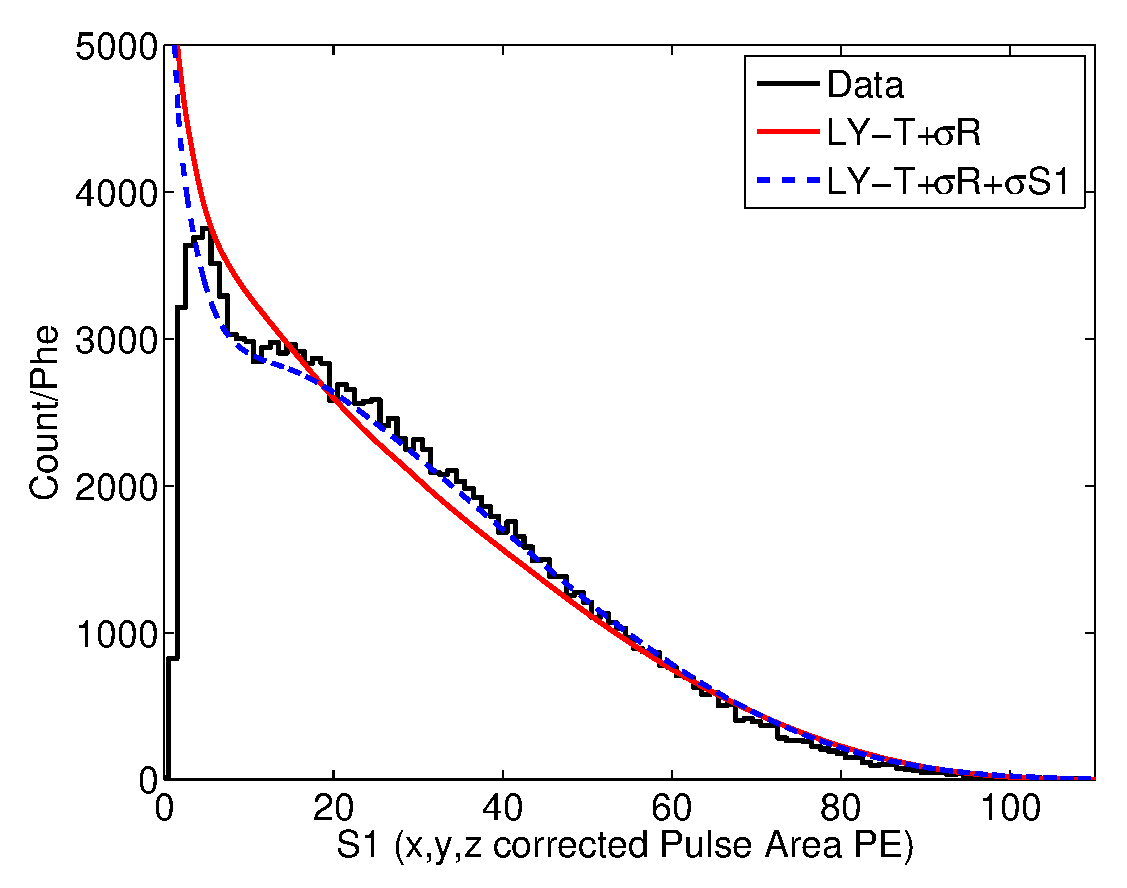
\includegraphics[width=73mm]{Chapter_Flucs/Figures/S1S2_Spectra/S1_spec_compare_iter1_.eps}}
\hfill
\subcaptionbox{$\rm n_e$, 170 V/cm \label{fig:5b}}{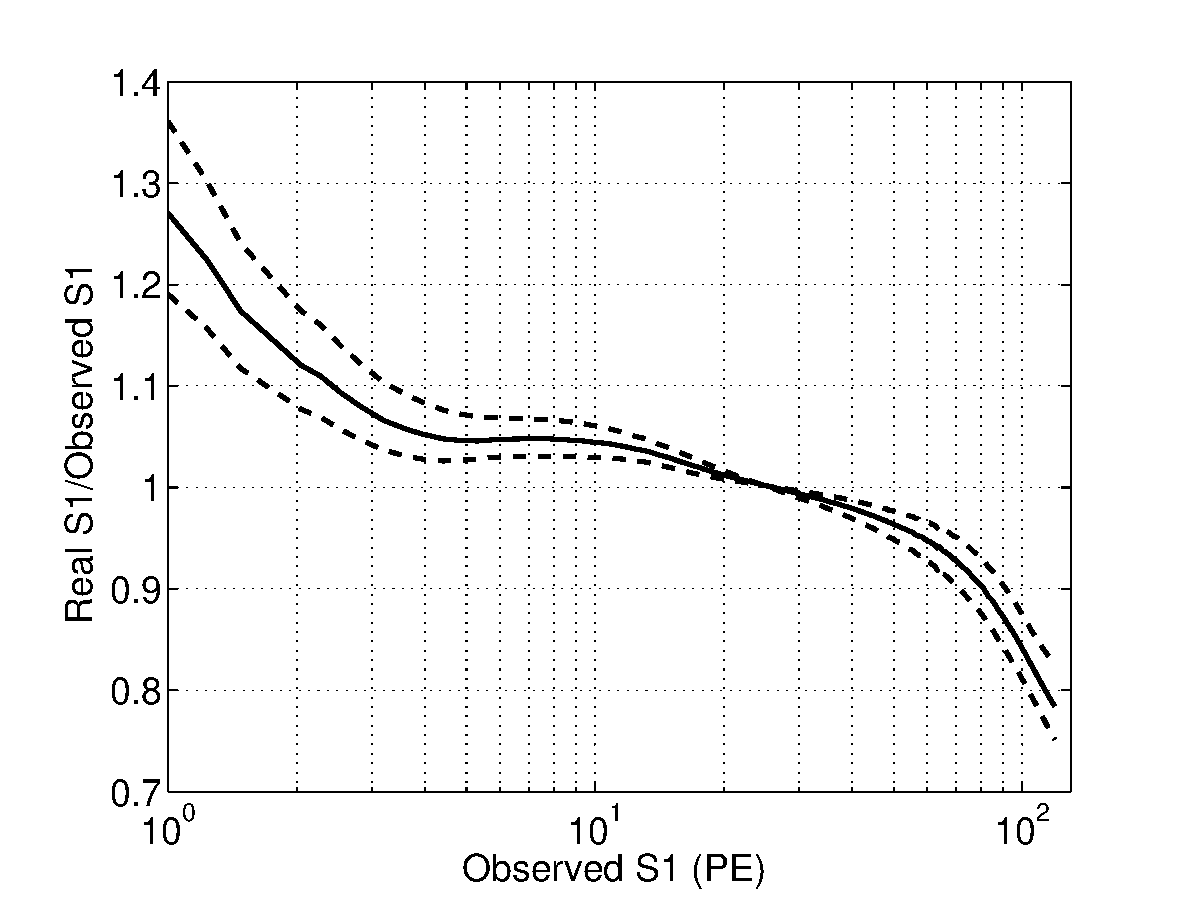
\includegraphics[width=73mm]{Chapter_Flucs/Figures/S1S2_Spectra/S1_corr_iter1_.eps}}

\bigskip

\subcaptionbox{$\rm n_\gamma$ 100 V/cm \label{fig:5c}}{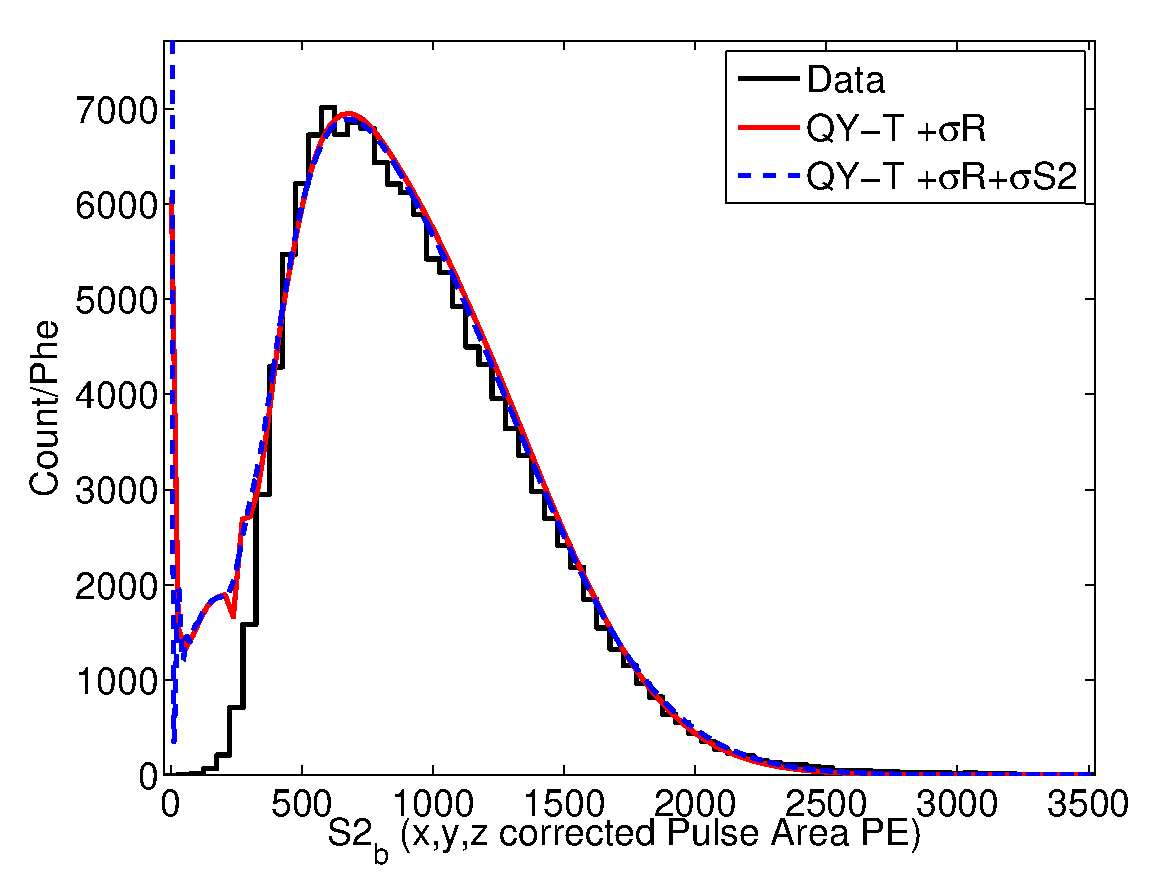
\includegraphics[width=73mm]{Chapter_Flucs/Figures/S1S2_Spectra/S2_spec_iter1_.eps}}
\hfill
\subcaptionbox{$\rm n_e$, 100 V/cm \label{fig:5c}}{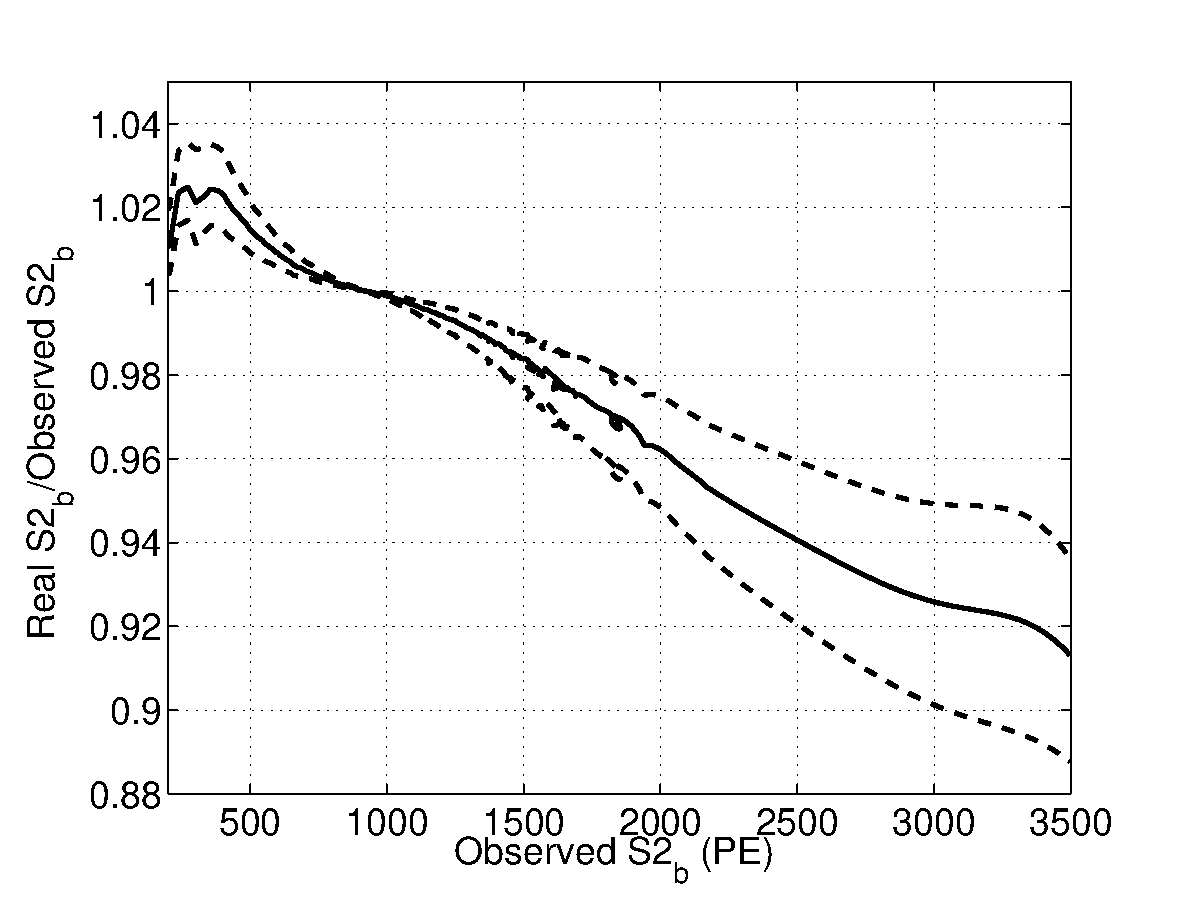
\includegraphics[width=73mm]{Chapter_Flucs/Figures/S1S2_Spectra/S2_corr_iter1_.eps}}

\caption{a): In Black S1 tritium S1 spectrum extracted from the data. In red, the S1 spectrum based upon the LY and QY measured from the tritium data after applying recombination fluctuations. In dashed blue, the expected S1 spectrum after applying finite detector resolutions of equation \ref{eq:S1_res}.  b): The ratio of the real mean to the observed mean vs. the observed mean after smearing the tritium photon spectrum with detector resolution. Note the S1 threshold at about 3 PE in S1. c): In black, tritium S2 spectrum from the data. In red, the S2 spectrum based upon the LY and QY measured from the tritium data after applying recombination fluctuations. In dashed blue, the expected S2 spectrum after applying finite detector resolutions of equation \ref{eq:S2_res}. d): The ratio of the real mean to the observed mean vs. the observed mean after smearing the tritium electron spectrum from NEST with detector resolution. Note the S2 threshold at about 400 PE in S2.   }
\label{fig:S1S2_mapping_2}
\end{figure}
\renewcommand{\baselinestretch}{2}
\small\normalsize


As expected, we find good agreement between the smeared tritium S1 and S2 spectra with the data. The spectral shape correction found for both S1 and S2 is consistent with those found by using NEST previously, shown in figure \ref{fig:S1S2_mapping_2}. This gives us confidence that we can apply the mapping of true mean to observed to the data. 

The meaning of the spectral shape corrections for S1 and S2 shown in figure \ref{fig:S1S2_mapping_2} (b) and (d) can be understood as a mixture of spectral shape and varying resolution. As the measured value of S1 drops to 1 PE (20\% detection efficiency) we find the correction factor rises to a factor of 1.3. Even though the count rate is growing in lower S1 bins the narrowing S1 resolution cancels out the spill over from lower S1s as compared to the overlap from larger S1s with a lower count. This effect causes an observed S1 mean of 1 PE to actually be comprised of events with a mean of 1.3 PE. On the other end the correction is straight forward. As the beta spectrum is dropping sharply to reach 0 at the Q value of 18.6 keV \cite{Tritium_Q} events from the more populated lower energy bins spill over into higher energy regions. This effect causes the observed mean at the endpoint of 18.6 keV to actually be comprised of events with an average energy of 15 keV. Note, that the energy spectrum with detector resolution extends to 21-22 keV due to upward statistical fluctuations in S1 and S2. The S2 spectrum exhibits the same behavior at the high end above the peak of the spectrum around 1000 PE. As the S2 approaches threshold of 400 PE there is a $<$ 3\% correction to the mean to account for the spill over of the more populated regions to the right. This is different than case of S1 at low PE as the S2 resolution is about a factor of three better at the threshold.

\begin{comment}
%Put in chapter 7? Add LED data here?
\section{Detector Threshold Measured with Tritium}

By convolving the yields with the true tritium energy spectrum the S1 and S2 spectra extend below our energy threshold (50\% at 1 keV). The detection threshold for S1 and S2 can be determined by taking the difference between the data and the expected tritium spectra with recombination and detector resolution $\rm \sigma_R$, $\rm \sigma_{S1}$ and $\rm \sigma_{S2}$, figure \ref{fig:S1S2_mapping_2}. The energy threshold is also determined by taking the ratio of the data to the true tritium spectrum with detector resolution, showing in figure \ref{fig:E_spec}. The following two figures show the results of S1 and S2 and energy thresholds at 170 V/cm in and at 100 V/cm in figure \ref{fig:Thres}.

\begin{figure}[h!]\centering
 
\subcaptionbox{S1 \label{fig:3a}}{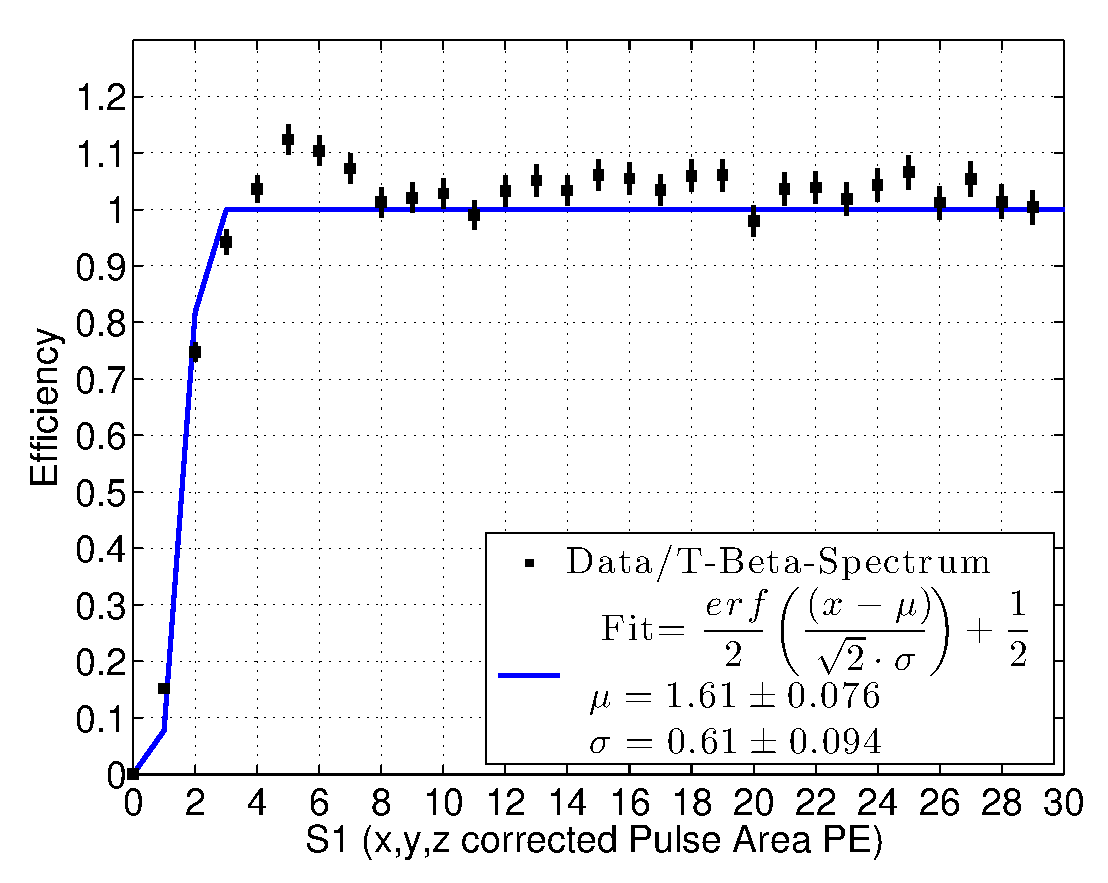
\includegraphics[width=70mm]{Chapter_Flucs/Figures/S1S2_Spectra/S1_Thres_.eps}}
\hfill
\subcaptionbox{$\rm S2_b$ (golden) \label{fig:3b}}{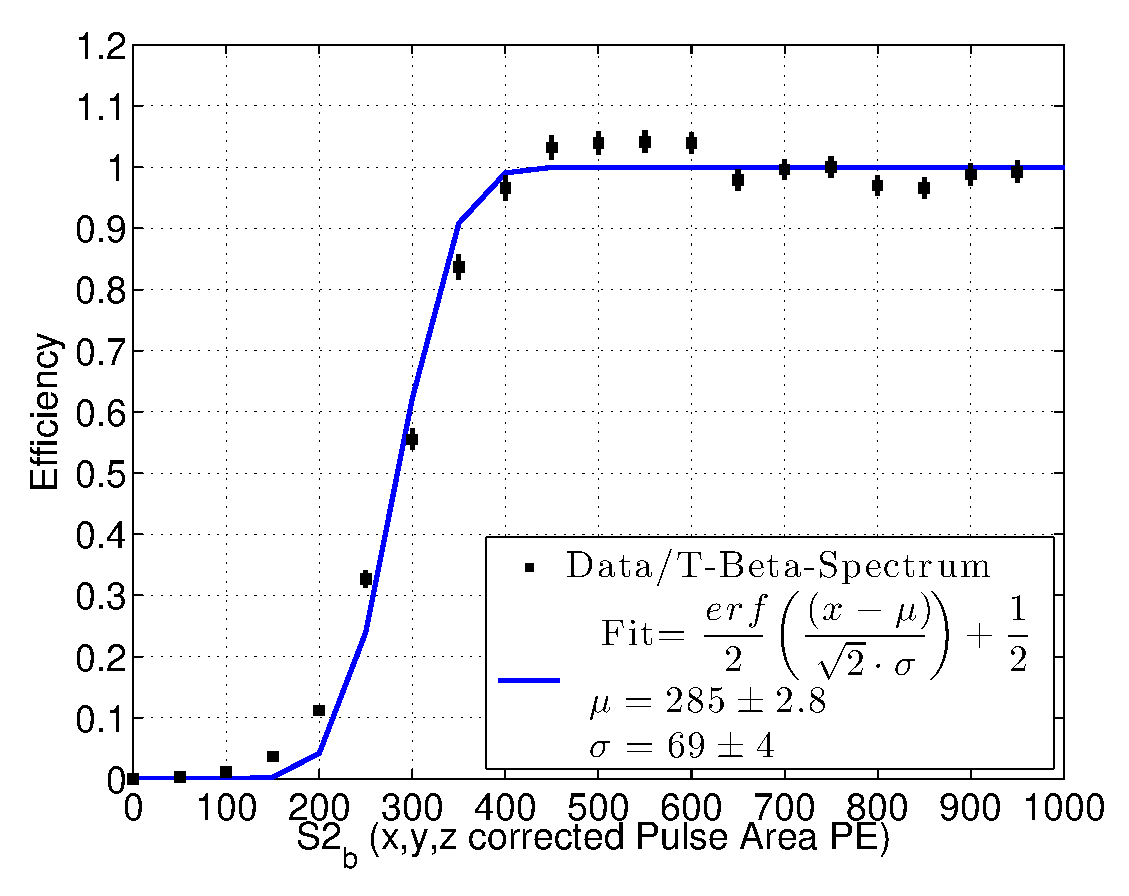
\includegraphics[width=70mm]{Chapter_Flucs/Figures/S1S2_Spectra/S2_Thres_.eps}}

\bigskip

\subcaptionbox{Combined Energy \label{fig:3c}}{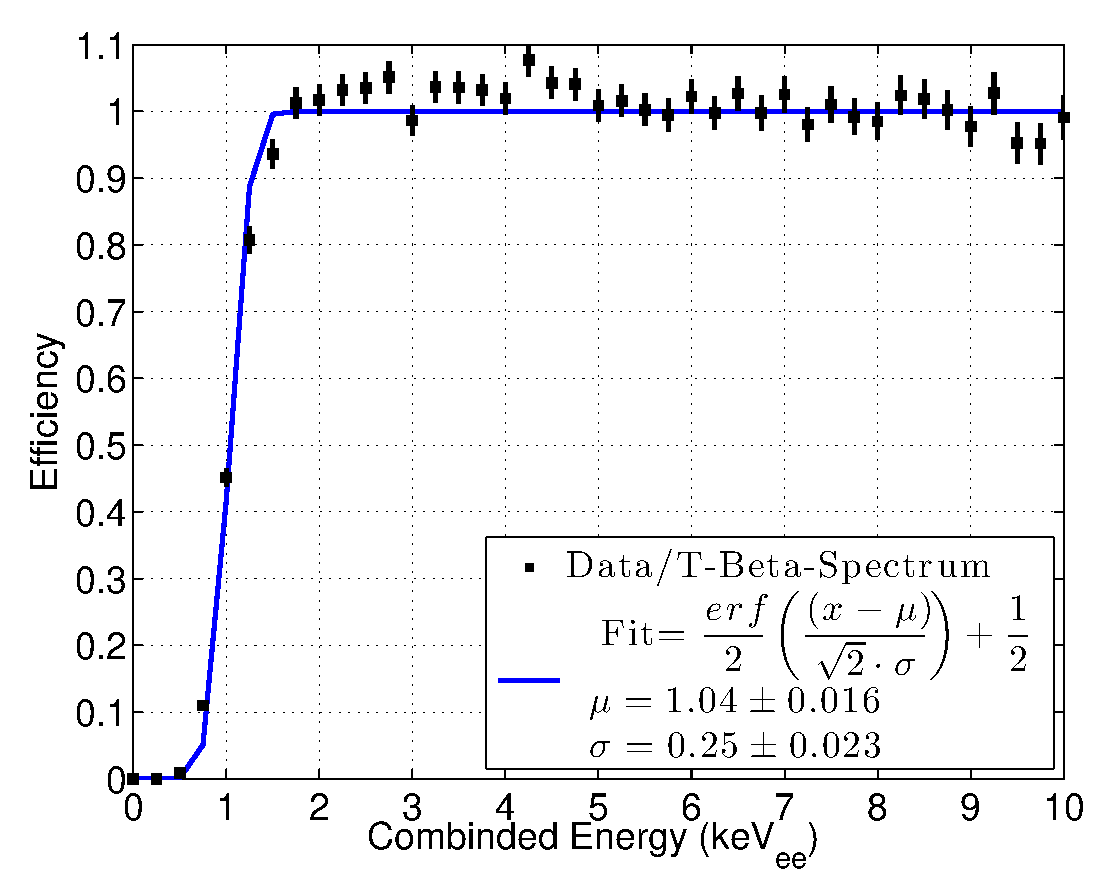
\includegraphics[width=70mm]{Chapter_Flucs/Figures/E_Spec/E_Thres_LY_QY_iter1.eps}}

\caption{Threshold calculated from difference of simulated Tritium S1, S2 and energy spectra. a) S1 b) $\rm S2_b$, c) Energy . The data set contained 140,000 tritium events in the fiducial}
\label{fig:Thres}
\end{figure}


\begin{figure}[h!]\centering
 
\subcaptionbox{S1 \label{fig:3a}}{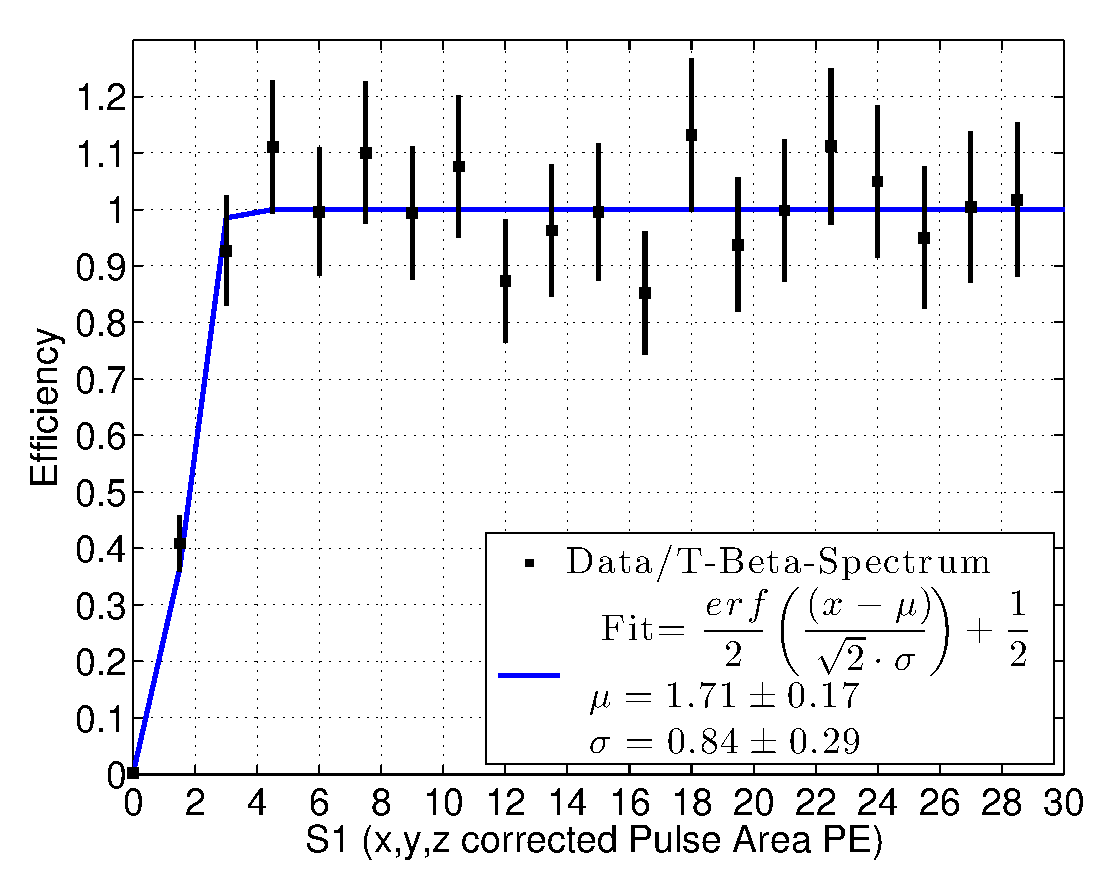
\includegraphics[width=70mm]{Chapter_Flucs/Figures/Spec_Thresh_100/S1_Thres_.eps}}
\hfill
\subcaptionbox{$\rm S2_b$ (golden) \label{fig:3b}}{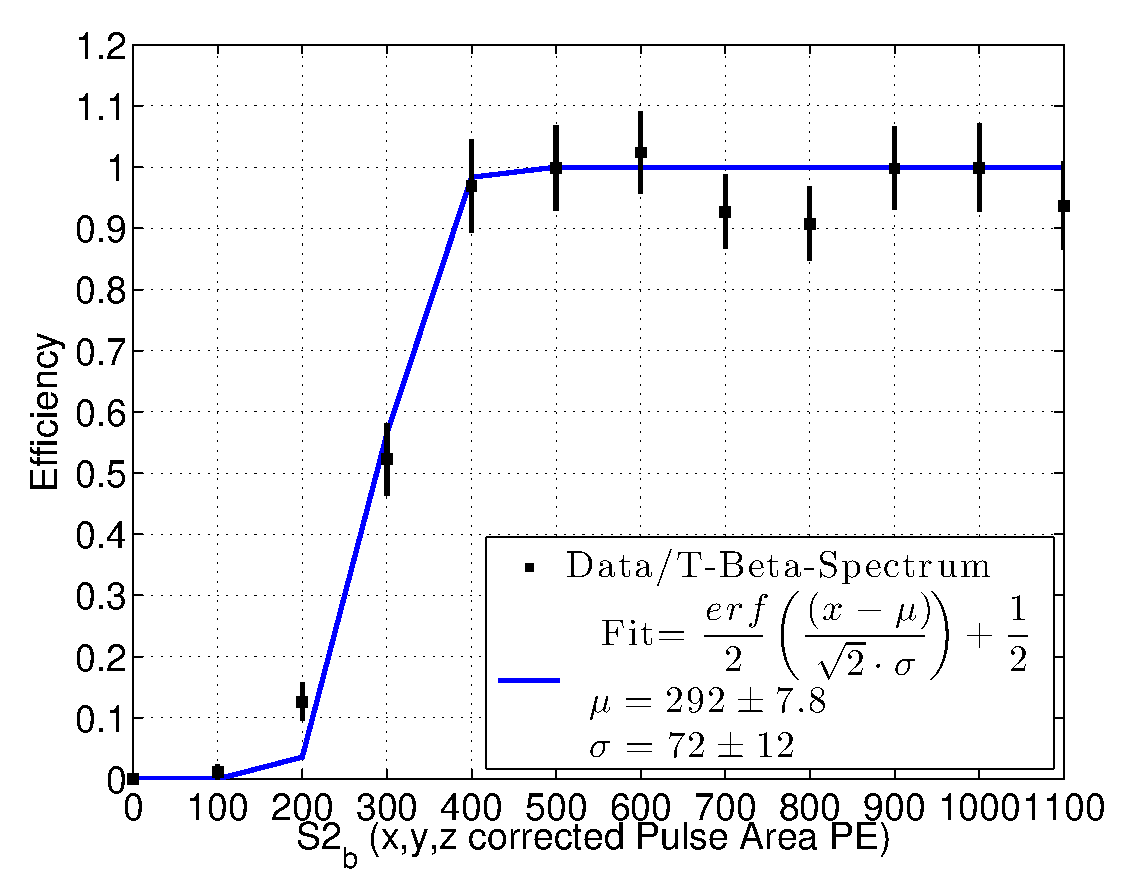
\includegraphics[width=70mm]{Chapter_Flucs/Figures/Spec_Thresh_100/S2_Thres_.eps}}

\bigskip

\subcaptionbox{Combined Energy \label{fig:3c}}{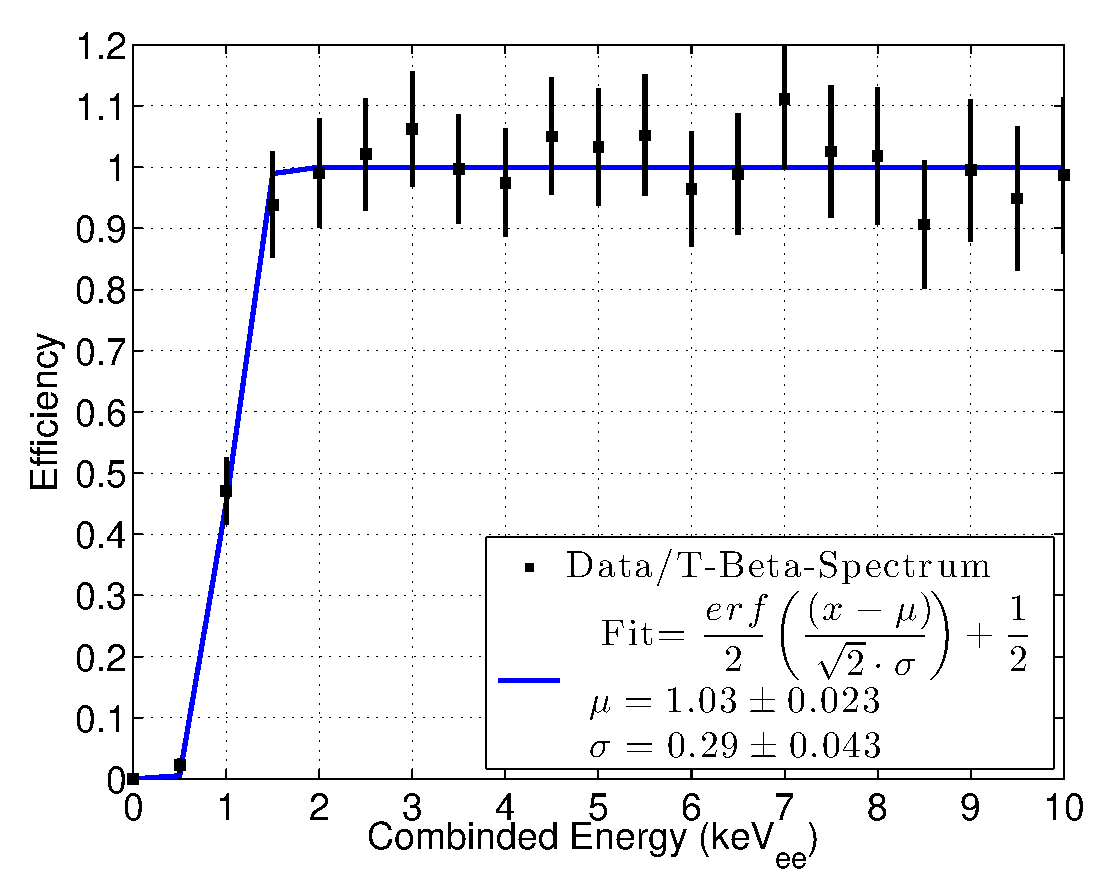
\includegraphics[width=70mm]{Chapter_Flucs/Figures/Spec_Thresh_100/E_Thres_.eps}}

\caption{Threshold calculated from difference of simulated Tritium S1, S2 and energy spectra at 100 V/cm. a) S1 b) $\rm S2_b$, c) Energy . The data set contained 2,500 tritium events in the fiducial.}
\label{fig:Thres_100}
\end{figure}

\newpage

The energy threshold  in the WIMP search is set by the ability to detect the much smaller S1 signal. For both the case of 100 V/cm and 170 V/cm the  detection efficiency for golden events at 2 PE is 80\%. Surprisingly, the energy threshold is found to be insensitive to the difference in fields of 100 and 170 V/cm. The expectation was that at the higher field the charge yield would increase leading to less recombination, lower light yield and thus a lower energy threshold. However, as seen in figure \ref{fig:R_T}, recombination at the two fields merges below 4 keV, leading to identical threshold and discrimination. There appears to be little benefit in threshold or discrimination (ER band mean) between from 100 to 170 V/cm. At higher fields the effect is expected to be more noticeable \cite{NEST_2013}.

\end{comment} % removed threshold discussion for Chapter 7.

\newpage

\section{Ionization and Scintillation Yield After Correction}

The light and charge yield which can now be extracted from the tritium data are unique properties of liquid xenon given for ER interaction at low energies. Figure \ref{fig:LYQY_data} shows the data used to calculate the means after having corrected for the S1 and S2 spectral shape. Two tritium calibration data sets are shown, one with high statistics at 170 V/cm containing 140,000 events and the second at 100 V/cm with a modest 2,500 events. (Both numbers correspond to events in the fiducial volume).
 
 %Above 10 keV yields from betas and gammas begin to deviate by several percent \cite{NEST} \cite{NEST_2013}.
 
%LY QY and stat, raw data

\renewcommand{\baselinestretch}{1}
\small\normalsize
\begin{figure}[h!]\centering
 
\subcaptionbox{$\rm n_\gamma$, 170 V/cm \label{fig:5a}}{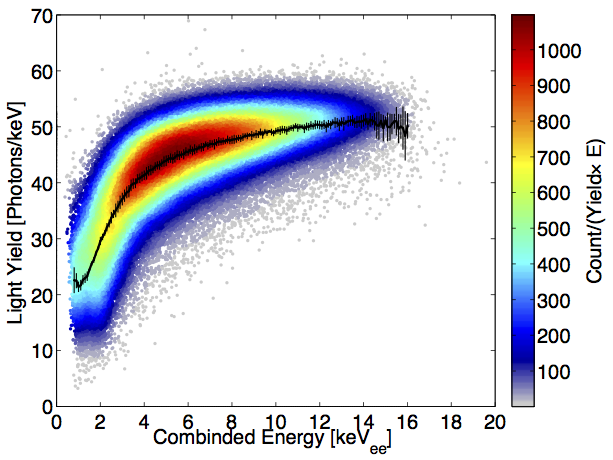
\includegraphics[width=73mm]{Chapter_Flucs/Figures/LYQY_Iter1/LY_c_180_means_.png}}
\hfill
\subcaptionbox{$\rm n_e$, 170 V/cm \label{fig:5b}}{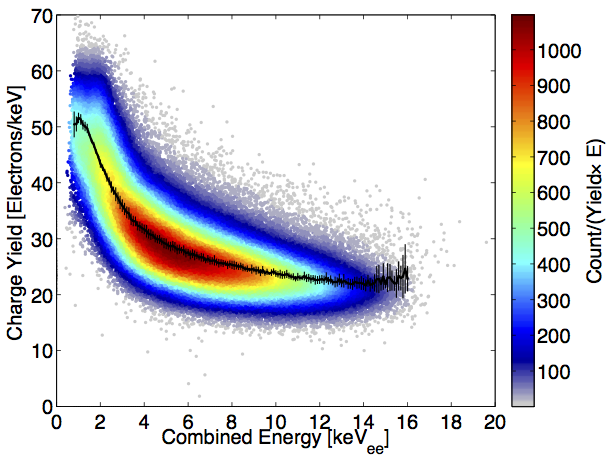
\includegraphics[width=73mm]{Chapter_Flucs/Figures/LYQY_Iter1/QY_c_180_means_.png}}

\bigskip

\subcaptionbox{$\rm n_\gamma$ 100 V/cm \label{fig:5c}}{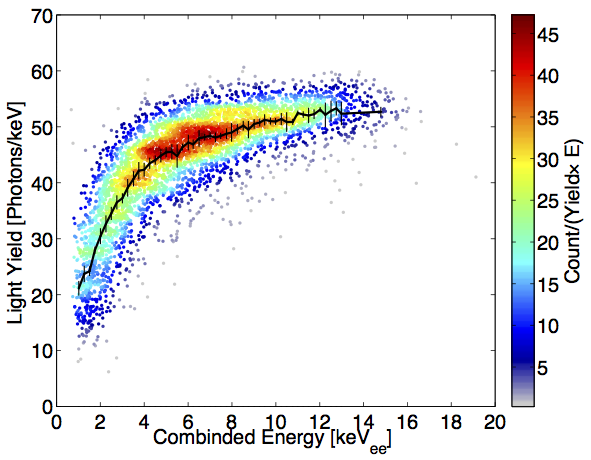
\includegraphics[width=73mm]{Chapter_Flucs/Figures/Iter1_100/LY_c_100_means_.png}}
\hfill
\subcaptionbox{$\rm n_e$, 100 V/cm \label{fig:5c}}{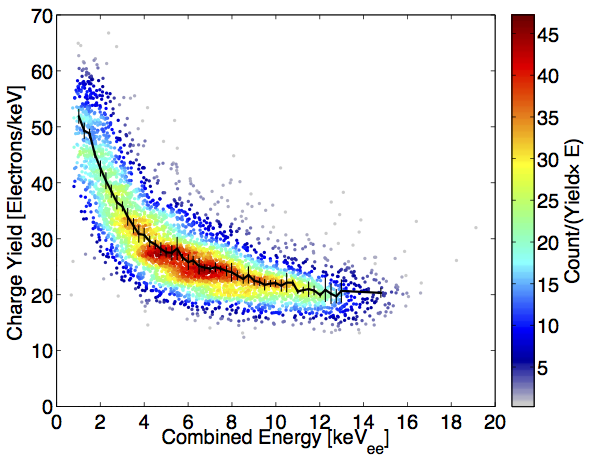
\includegraphics[width=73mm]{Chapter_Flucs/Figures/Iter1_100/QY_c_100_means_.png}}

\caption{Means of the light yield and charge yield from tritium data corrected for spectral shape along with the 1 sigma statistical errors.}
\label{fig:LYQY_data}
\end{figure}
\renewcommand{\baselinestretch}{2}
\small\normalsize

The means used for LY and QY are the population means in each slice of energy for our best value of g1 and g2. The errors shown are the statistical errors along with a small systematic component from the difference of the population mean from the Gaussian mean. The systematic offset from the constraint of g1 and g2 are treated in figure \ref{fig:LYQY_iter1}. With the potential for tighter constraints on the value of gains g1 and g2, the remaining uncertainty in the measurement of LY and QY would be less than 3\% below 10 keV. The tritium calibration source has the potential to be used to determine the light and charge yield in liquid xenon to less than 3\% including at the detector threshold. This calibration source hold great promise considering that few yield measurements exist below 5 keV. 

Figure \ref{fig:LYQY_iter1} shows the mean yields with the one sigma bands from the uncertainty in gains g1 and g2. The errors are anti-correlated, thus a shift up in light yields corresponds to a shift down in charge yield preserving the energy. The figure also shows the one sigma prediction of the yields from NEST \cite{NEST_2013} shaded in blue where the model is interpolated and magenta where the model is extrapolated. 


\renewcommand{\baselinestretch}{1}
\small\normalsize
\begin{figure}[p!]\centering
 
\subcaptionbox{$\rm n_\gamma$, 170 V/cm \label{fig:5a}}{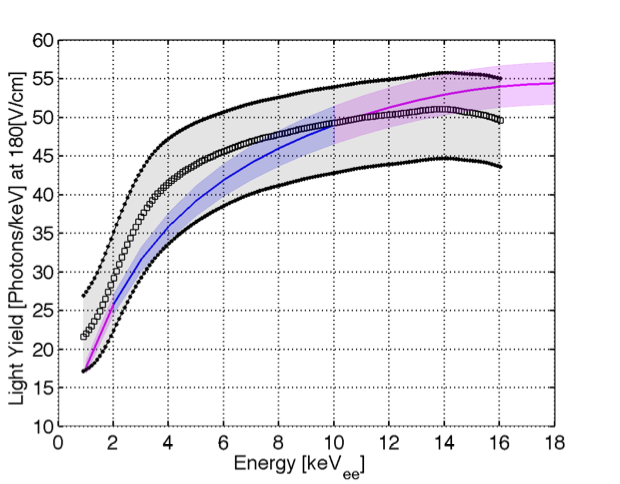
\includegraphics[width=73mm]{Chapter_Flucs/Figures/LYQY_iter1/LY_180_iter1_1sigBand_.png}}
\hfill
\subcaptionbox{$\rm n_e$, 170 V/cm \label{fig:5b}}{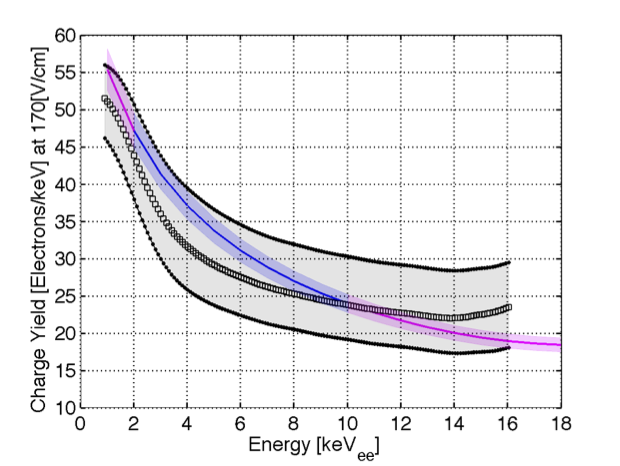
\includegraphics[width=73mm]{Chapter_Flucs/Figures/LYQY_iter1/QY_180_1sigBand_.png}}

\bigskip

\subcaptionbox{$\rm n_\gamma$ 100 V/cm \label{fig:5c}}{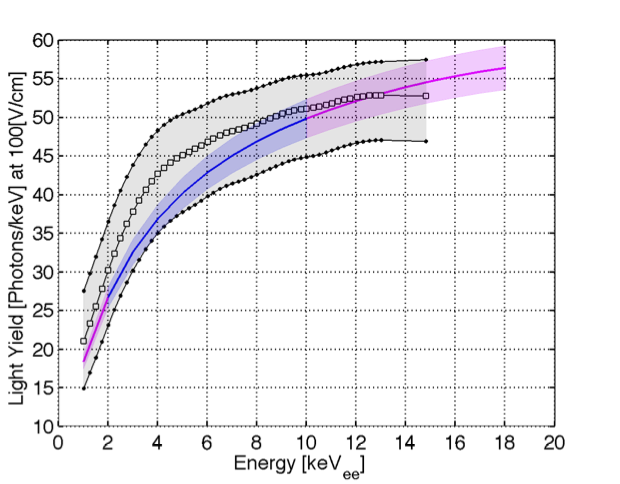
\includegraphics[width=73mm]{Chapter_Flucs/Figures/LYQY_iter1/LY_100_iter1_1sigBand_.png}}
\hfill
\subcaptionbox{$\rm n_e$, 100 V/cm \label{fig:5c}}{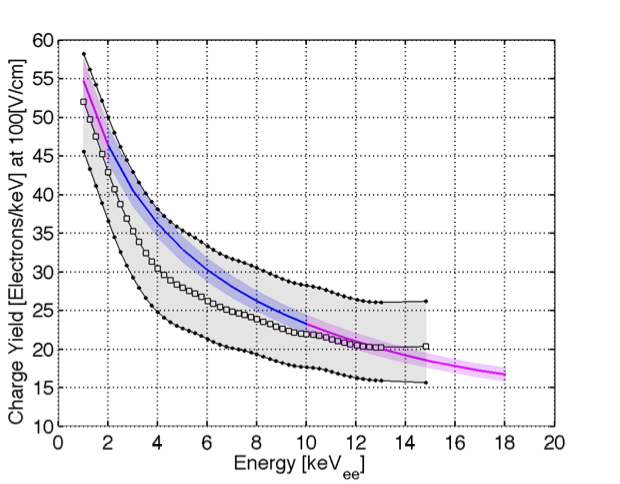
\includegraphics[width=73mm]{Chapter_Flucs/Figures/LYQY_iter1/QY_100_iter1_1sigBand_.png}}

\caption{Light yield and charge yield from tritium data corrected for spectral shape along with the 1 sigma systematic constraint on g1 and g2. The blue and magenta curve are NEST extrapolation and interpolation, respectively.}
\label{fig:LYQY_iter1}
\end{figure}
\renewcommand{\baselinestretch}{2}
\small\normalsize


%The means are not surprisingly off from the NEST predictions which is what lead to the initial discrepancy in the S1 and S2 spectra.
The overlap between the data and the NEST model is within one sigma considering errors in g1 and g2. However, as the errors in g1 and g2 are systematic and 100\% correlated bin-to-bin they can only shift the curves up or down. Even under such a shift, the shape of the tritium data would not agree perfectly with the NEST prediction. As the statistical uncertainty alone constrains the means to better than 3\% below 10 keV for the 170 V/cm data set. 

%% Compare Before and after spectral shape correction. Spectral_Shape_Comp
\newpage
The comparison of measured light and charge yield before and after the tritium spectral shape correction is shown in figure \ref{fig:LYQY_iter1_comp} . The band in red is the result from using the raw data and combined energy, the band shown in blue is after the correction. The yields before and after the correction overlap with the exception of the last 15-18 keV bins which are pulled back as the events reconstructed at those energies on average were the result of events with 20\% less energy, having upward fluctuated. In the middle regions however the spectral shape correction of the energy, the photon (S1) and electron (S2) spectrum are canceled. Recalling that yield is defined as $\rm n_\gamma/E $, and $\rm n_e/E$, with $\rm E=W(n_\gamma + n_e)$. Thus, on average the upward or downward fluctuations in collected photons and electron are canceled by the corresponding fluctuations in reconstructed energy E.

\renewcommand{\baselinestretch}{1}
\small\normalsize
\begin{figure}[p!]\centering
 
\subcaptionbox{$\rm n_\gamma$, 170 V/cm \label{fig:5a}}{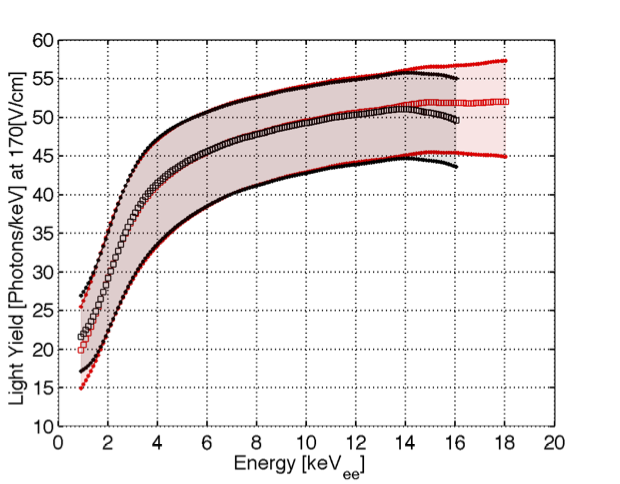
\includegraphics[width=73mm]{Chapter_LYQY/Spectral_Shape_Comp/LY_170_iter1_comp.png}}
\hfill
\subcaptionbox{$\rm n_e$, 170 V/cm \label{fig:5b}}{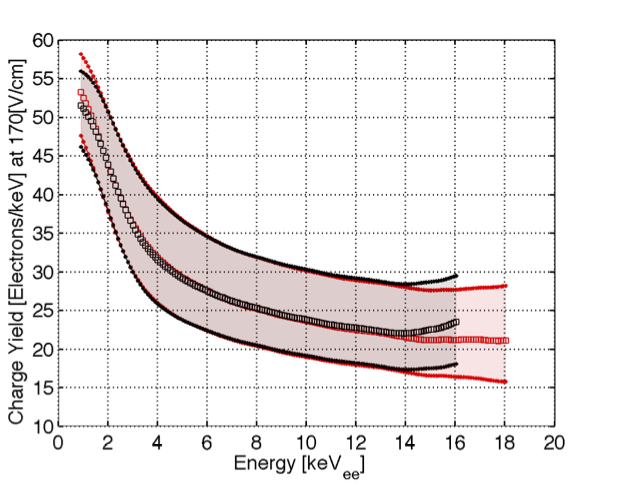
\includegraphics[width=73mm]{Chapter_LYQY/Spectral_Shape_Comp/QY_170_iter1_comp.png}}

\bigskip

\subcaptionbox{$\rm n_\gamma$ 100 V/cm \label{fig:5c}}{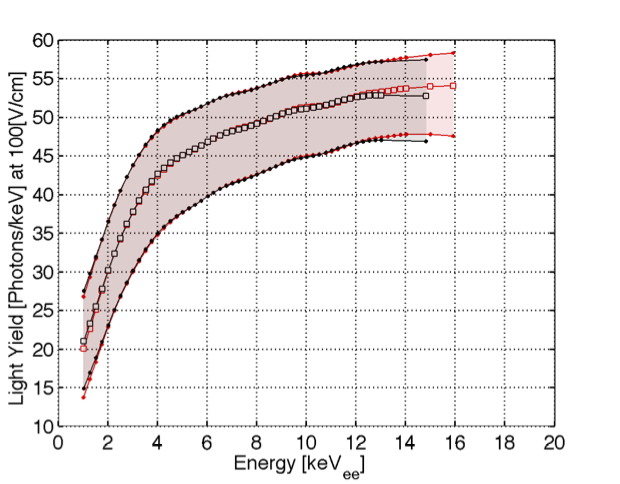
\includegraphics[width=73mm]{Chapter_LYQY/Spectral_Shape_Comp/LY_100_iter1_comp.png}}
\hfill
\subcaptionbox{$\rm n_e$, 100 V/cm \label{fig:5c}}{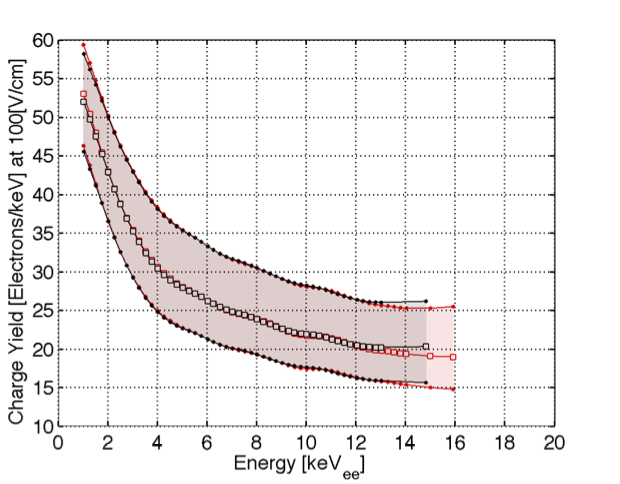
\includegraphics[width=73mm]{Chapter_LYQY/Spectral_Shape_Comp/QY_100_iter1_comp.png}}

\caption{In black, the light yield and charge yield from tritium data corrected for spectral shape. In red, the light yield and charge yield from tritium data uncorrected for spectral.  The shaded region represent the one sigma systematic error from the constraint on g1 and g2 shaded. }
\label{fig:LYQY_iter1_comp}
\end{figure}
\renewcommand{\baselinestretch}{2}
\small\normalsize



%Using the tritium data we can improve the model, which is crucial for characterizing the backgrounds of any liquid xenon detector in the WIMP search region of several keV. The yields when convolved with energy spectral produce the expected ER band from a given background source.
One question remaining to be answered is if the yields and ER band defined by tritium beta decays are consistent with the more generic Compton Scatter backgrounds, which are expected to be found in the WIMP search data. It is expected that betas and gammas are indistinguishable below 10 keV \cite{NEST} \cite{NEST_2013}. In the following section we will compare the light yield results from the tritium data with recent Compton scattering measurements that have probed light yield in xenon down to 1.5 keV. 

%For LUX roughly 2/3 of ER background below 5 keV are Compton scatters and 1/3 are betas from $\rm^{85}Kr$.



\newpage

\section{Comparison of Light Yield Measured With Tritium to Other Measurements With Compton Scatters}

In this section we compare the LY measured with tritium in LUX to that measured with Compton scatters by other researchers.
When comparing measurements from different xenon detectors it is prudent to report the result relative to that of a standard calibration source. The light yields reported for low energy Compton scatter measurements from  \cite{Baudis} \cite{Aprile_LY} are normalized to the first 32.1 keV decay of \KrCal. Before comparing the light yields results from the tritium calibration we first need to measure the light yield in LUX at zero field from \KrCal.

\subsection{The Standard Candle: Light Yield from $\rm^{83m}Kr$}

%Quenching of scintillation yield vs. field has been  typically defined relative to 32.1 keV decay of $\rm^{83m}Kr$ at zero field \cite{Aprile_LY},\cite{Baudis}. 

The \KrCal source was discussed in greater in chapter \ref{Ch:3}. The decay of \KrCal consists primarily of the emission of two internal conversion electrons at 32.1 keV and 9.4 keV, with a half life of 154 ns between the two \cite{Kastens} \cite{83Kr_HalfLife_1} \cite{83Kr_HalfLife_2} . The combined signal (41.6 keV) is found by the LUX pulse finder in the majority of cases. However, the combined signal is not useful as a standard calibration. The second 9.4 keV decay receives an enhancement in light yield due to increased recombination probability from the the presence of ions and electrons from the initial 32.1 keV decay. It has been observed that the light yield enhancement depends upon the decay time separation, out to 1000 ns \cite{Kastens} and \cite{Baudis}. In the LUX detector we have also observe the enhancement of the light yield of the second 9.4 keV out to 2000 ns shown in figure \ref{fig:Yield_Kr9}. Our ability to split pulses with 100\% efficiency starts at 1200 ns.

 \begin{figure}[h!]\centering
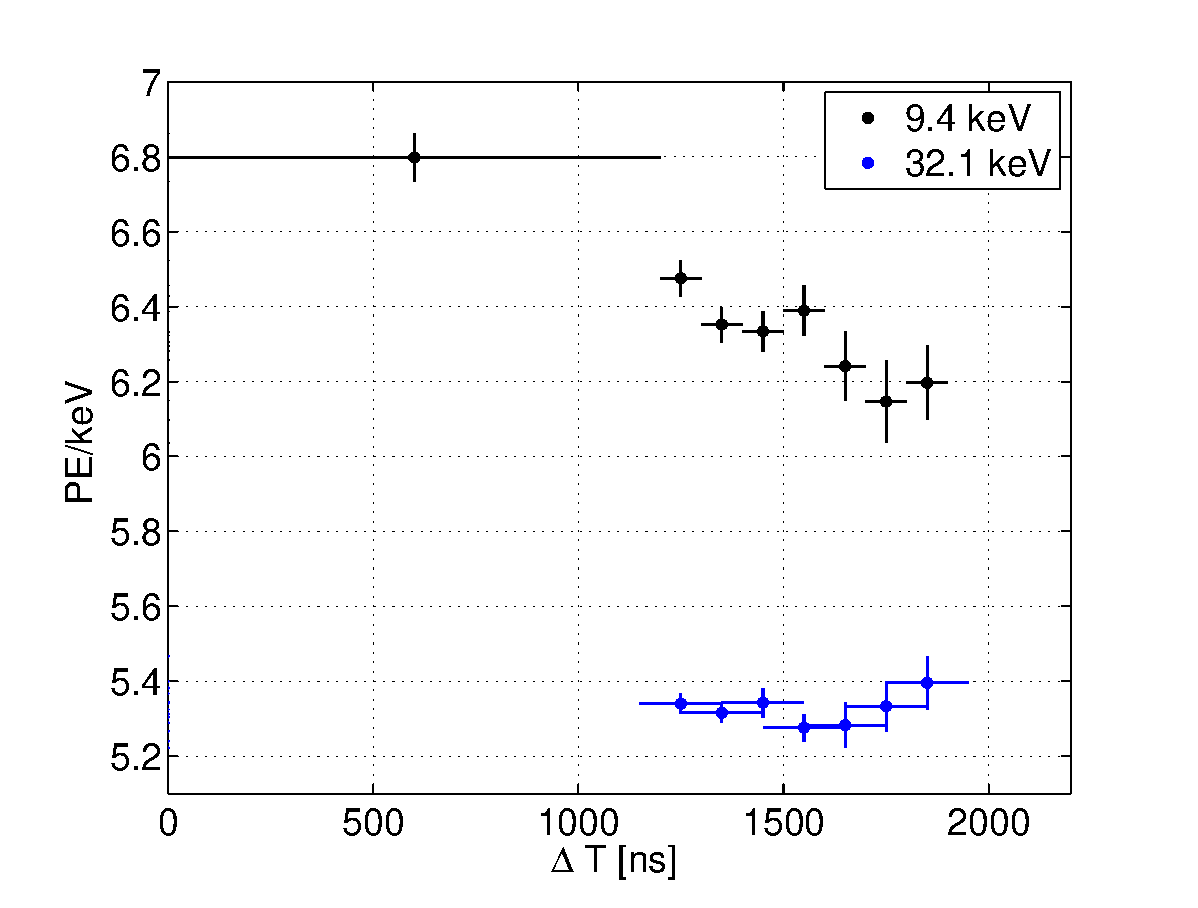
\includegraphics[width=73mm]{Chapter_Flucs/Figures/Kr/dT_lux10_20130510T1250_cp09323} %old cp 6914
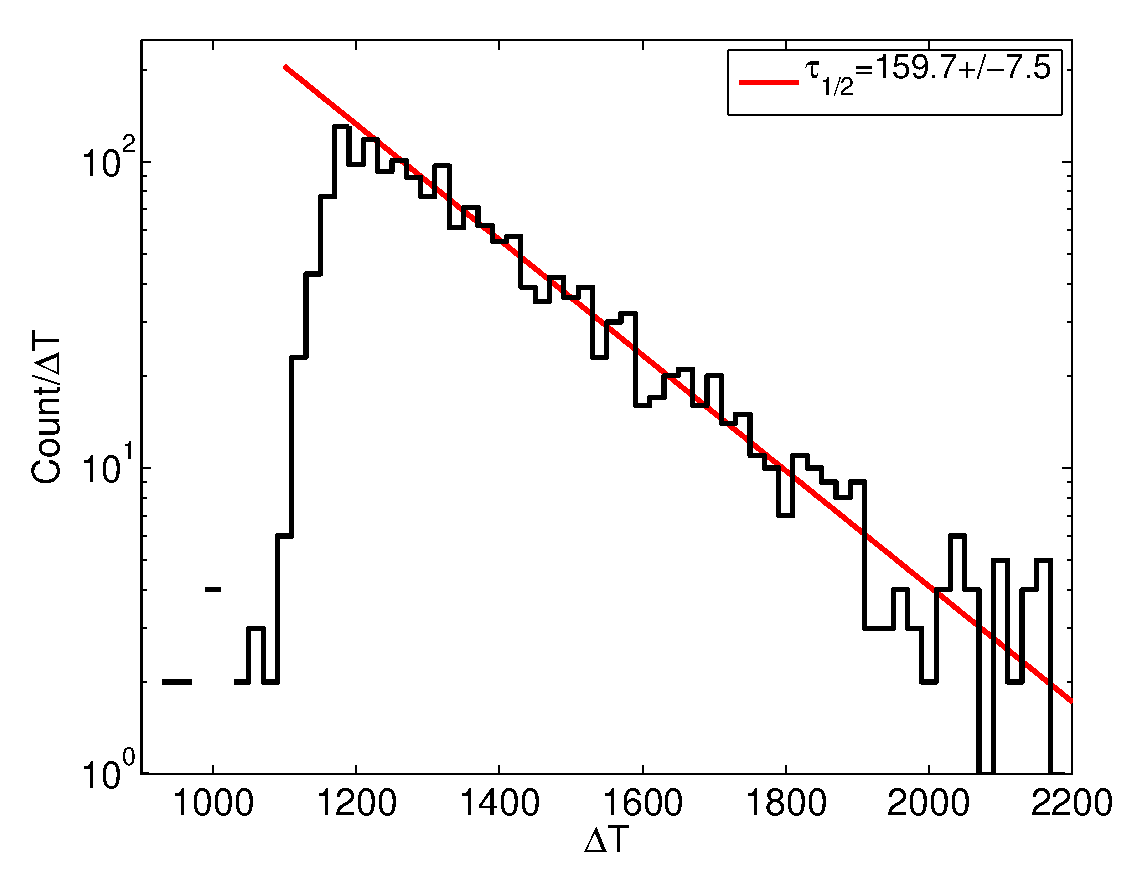
\includegraphics[width=73mm]{Chapter_Flucs/Figures/Kr/dT_fit_lux10_20130510T1250}
\caption{Left: The light yields of the 9.4 and 32.1 keV decay of \KrCal plotted vs. timing separation, for events separated by more than 1200 ns. The point at 600 ns is calculated assuming the 32.1 keV yield remains flat to 200 ns as observed in \cite{Kastens} and \cite{Baudis} . Right: the histogram of \KrCal events vs timing separation finding a best fit to the half life of 159.7 $\pm$ 7.5 consistent with the measured value of 154 ns \cite{83Kr_HalfLife_1} \cite{83Kr_HalfLife_2}. }
\label{fig:Yield_Kr9}
\end{figure}

Fortunately, the first 32.1 keV appears to have no time dependence as it decays under normal circumstances in the xenon, without the presence of additional free ions or electron \cite{Baudis}, \cite{Aprile_LY}. Using a $\rm^{83m}Kr$ data set at zero field the yield of the 32.1 keV decay was determined. Since the S2 (charge) signal is unavailable at zero drift field we rely on the the top-bottom asymmetry of the PMTs to define the Z coordinate of the event, $\frac{top-bottom}{top+bottom} $. We must know at least the Z coordinate in order to apply the position dependent corrections outlined in chapter \ref{Ch:3}. The XY correction is subdominant to the Z-dependent correction for the S1 signal and can be ignored. Each event, given a top-bottom asymmetry, is mapped to a detector depth Z allowing for the Z-dependent correction to be applied. The correction normalizes the pulse area PE to the detector center (241.6 mm below the gate grid). The result for the zero field data set is shown in figure \ref{fig:ZeroField_Kr} and is reported in table \ref{table:kr32}.
 
 \begin{figure}[h!]\centering
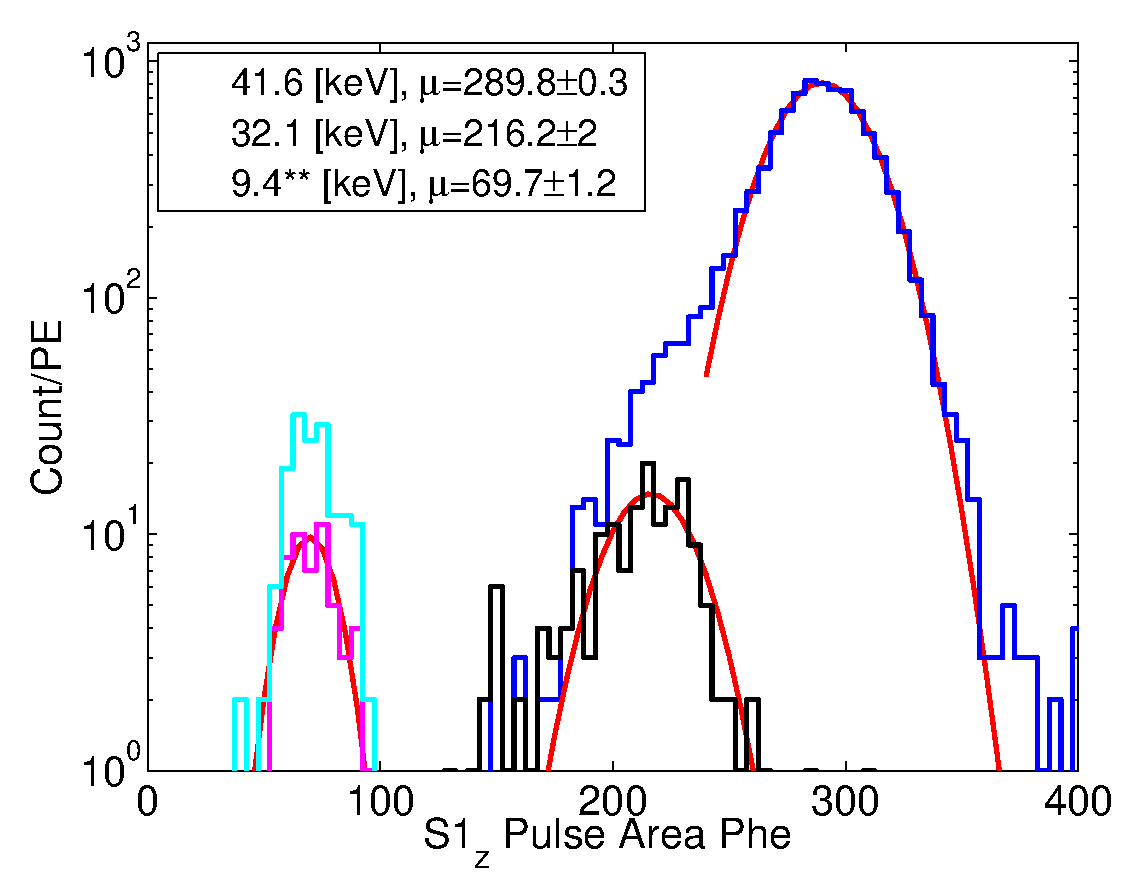
\includegraphics[width=72mm]{Chapter_Flucs/Figures/S1_Z_no_field_lux10_20131009T1358_cp09670} %old cp 6914
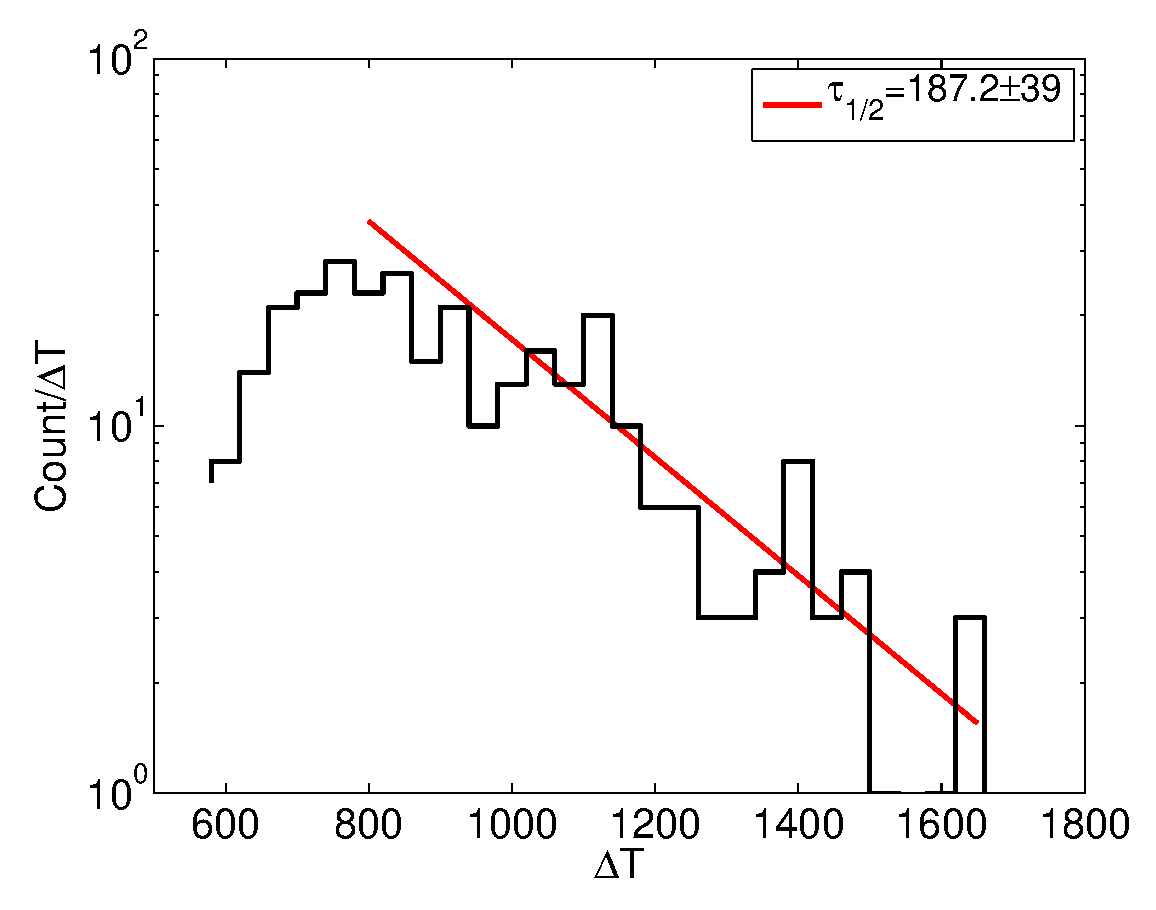
\includegraphics[width=72mm]{Chapter_Flucs/Figures/dT_no_field_2lux10_20131009T1358_cp09670}
\caption{Left: S1 $\rm^{83m}Kr$ peaks at zero field. Right: shows the histogram of the separated 32.1 and 9.4 keV decays plotted above vs. time. The half life fit to the population is in good agreement with the measured half-life of 154 ns \cite{83Kr_HalfLife_1} \cite{83Kr_HalfLife_2}. }
\label{fig:ZeroField_Kr}
\end{figure}

Table \ref{table:kr32} shows the measured scintillation of the 32.1 keV internal conversion electron from $\rm ^{83m}Kr$ using the LUX detector at various fields. The table also includes the NEST predictions \cite{NEST_2013}. Electron mobility and charge separation at the interaction site increases with drift field leading to less recombination, causing scintillation yield to be quenched. The field effect is more dramatic at higher energies than in the low energy regions probed by the tritium data.

\renewcommand{\baselinestretch}{1}
\small\normalsize
\begin{table}[h!]
\begin{center}
\begin{tabular}{|c|c|c|c|c|c|}
\hline
Field	&S1			& Photons						& Yield 								&NEST	 \\
V/cm	& PE					& $\left<n_{\gamma}\right>$		& $\left<n_{\gamma}\right>$/keV	& $\left<n_{\gamma}\right>$/keV \\ \hline
0 		&	216.2 $\pm$ 5.0 	&2228.9 $\pm$ 50.5 &	69.4 $\pm$	1.6 	&	64.2 $\pm$ 3.2  \\ \hline
50 		&	195.0 $\pm$ 0.7 	&2010.3 $\pm$ 7.2   & 	62.6 $\pm$	0.2	&	59.8 $\pm$ 3.0 \\ \hline
100 	&	178.4 $\pm$ 0.7 	&1839.2 $\pm$ 	7.2	 &	57.3 $\pm$ 0.2 	&	55.8 $\pm$ 2.8 \\ \hline
170 	&  171.4 $\pm$ 0.9		&1767.0 $\pm$ 	9.2  &	55.0 $\pm$ 0.3 	&	51.9 $\pm$ 2.6 \\ \hline
\end{tabular}
\caption{Field dependence of the light yield form the 32.1 keV decay of $\rm^{83m}Kr$ along with the NEST \cite{NEST_2013} predictions.}
\label{table:kr32}
\end{center}
\end{table}
\renewcommand{\baselinestretch}{2}
\small\normalsize


\subsection{Comparing Tritium Scintillation Yield with Compton Scatters}

We report the measured light yield of tritium relative to the 32.1 keV decay of \KrCal at zero field, defined as $\rm \mathcal{R}_e$. The comparison is done as a proof of principle that the light yield from betas and gammas overlap at low energies, at least within the rather large systematic uncertainties. Further, this is a cross check that the residual $<$ $\rm10\times10^{-12}$ g/g concentration of methane injected for the tritiated-methane calibration had negligible impact on the light yield, as expected from previous measurements with methane\cite{Kirill_Methane}. The result for $\rm \mathcal{R}_e$ is shown in figure \ref{fig:Re}, with the one sigma regions plotted as bands for the tritium data.

 \begin{figure}[h!]\centering
 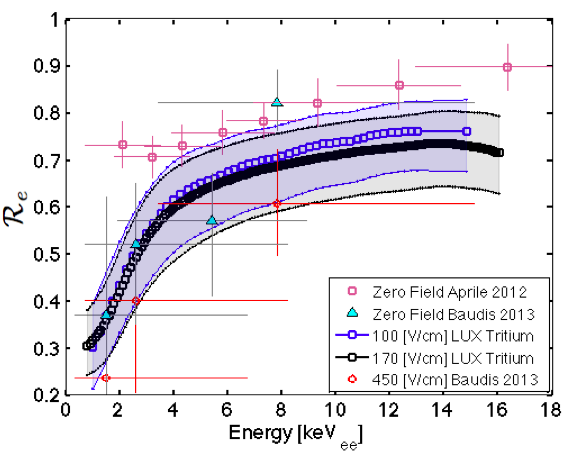
\includegraphics[width=150mm]{Chapter_Flucs/Figures/LYQY_iter1/Re_fig.png}
\caption{LY relative to the light yield of the 32.1 keV decay of \KrCal at zero field. The black and blue bands represent the results from tritium at 170 and 100 V/cm respectively. The shaded region represents the systematic error due to the one sigma constraints on g1 and g2.  Magenta points are Compton scattering measurements from \cite{Aprile_LY}. The gray and red represent zero field and 450 V/cm Compton Scattering measurements from \cite{Baudis}. }
\label{fig:Re}
\end{figure}

We find good agreement between the centroids of the tritium data at 100 and 170 V/cm with the zero field and 450 V/cm Compton scattering measurements from \cite{Aprile_LY} and \cite{Baudis}. The finding are consistent with the expectation that tritium light yield data at 100 and 170 V/cm lie between the zero field light yield measurements the light yield at 450 V/cm. The error bars from the Compton scattering measurement are rather large due to the uncertainty in scattering angle and the need for Monte Carlo to reconstruct the energy deposit in the liquid xenon. In those measurements, the combined energy of the deposit in the liquid xenon is uncertain as both experiments were done in light-only collection mode \cite{Aprile_LY}  \cite{Baudis} (even for the 450 V/cm measurement). The errors on the tritium results are systematic and dominated by the constraint of g1 and g2 and are comparable with the errors on the Compton scattering measurements. 

If the constraint on $\rm g_1$ and $\rm g_2$ in LUX is improved by future calibrations, then the errors on the tritium data will shrink significantly to below 3\% making the tritium calibration a powerful tool for calibrating both light yields and charge yields all the way to the energy threshold. The tritium light and charge yields reported here extend down to 1 $\rm keVee$ corresponding to the 50\% threshold of LUX. The measurements also confirm, within systematic errors, that the ER band as calibrated by the tritium data is applicable to the more generic Compton scatter backgrounds in the WIMP search region of 1 to 5 $\rm keV_{ee}$. Compton scatters comprises about 2/3 of the expected background in LUX with the remaining 1/3 being from the beta decay of $\rm ^{85}Kr$ \cite{LUX_BG}.


\section{Summery}

In this section we have extracted the light and charge yields using the tritium calibration source in energies ranging from 1 to 16 $\rm keV_{ee}$, shown in figures \ref{fig:LYQY_data} and \ref{fig:LYQY_iter1}. The light and charge yields measured are a fundamental property electronic recoils in liquid xenon, in this work the liquid density was 2.888 $\rm g/cm^3$. We find agreement, within the systematic errors, between the light yields measured with the tritiated-methane source with Compton scattering measurements down to 1.5 $\rm keV_{ee}$, figure \ref{fig:Re}. The result supports the model that low energy betas leave identical tracks to low energy Compton scatters in liquid xenon \cite{NEST} \cite{NEST_2013}. Having measured the yields, the S1 and S2 signals can be modeled for any background source only requiring the energy spectrum as an input. The ratio of charge (S2) to light (S1) characterizes a xenon detector's ability to reject background events from WIMP candidates at a particular energy. We have also found that the light and charge yields measured at 170 and 100 V/cm merge below 5 $\rm keV_{ee}$, indicating that below this energy recombination is insensitive to field. The results for ER and NR discrimination using the tritium calibration source will be discussed in the chapter \ref{Ch:T}.


%\begin{table}[h!]
%\begin{center}
%\begin{tabular}{|c|c|c|c|c|c|c|}
%\hline
%Field 	&41.6 keV 	& 32.1 keV 	& 9.4* keV 	&9.4** keV & S2	&S2 ** \\ 
% \[[V/cm]	&	S1PE	&S1PE	&S1PE&		S1PE		&S2PE		&S1PE  \\ \hline
%0 	&		359.9 $\pm$ 5	 			&267.4 $\pm$ 6.5 		&78 $\pm$ 2	 	&	 92.5$\pm$	6 		&	--  			& --	\\ \hline
%51 &		332.6 $\pm$ 1.4 			&246.7 $\pm$ 1.2 		&76.4 $\pm$ 0.5 	& 	86 $\pm$ 1		 &	3651 $\pm$ 5	& 3708 $\pm$ 11 \\ \hline
%105 &		316.8 $\pm$ 1.4 			&233.6 $\pm$ 1.4 		&72.9$\pm$ 0.5		 &	83 $\pm$ 1 			&	4357 $\pm$ &4399 $\pm$ 16 \\ \hline
%182	 & 		291.3 $\pm$ 1.4 			&212.3 $\pm$ 1.3		&68.8 $\pm$ 0.5 	&	79 $\pm$ 1 		&	4986 $\pm$ 5 	 &5048$\pm$ 13 \\ \hline
%\end{tabular}
%\caption{Field dependance of the light yield form the 32.1, 9.4 and combined 41.6 keV decay of $\rm^{83m}Kr$. The fields are calculated using a two dimensional model and not accounting potential charge accumulation on inner teflon panels. ** *}
%\end{center}
%\label{table:krAll}
%\end{table}